\documentclass[sigconf,authorversion]{acmart}

\graphicspath{{figures/}}

\usepackage[list=true, font=normalsize, labelfont=sf, labelformat=brace, position=top]{subcaption}
\usepackage[switch]{lineno}
\usepackage{csquotes}
\usepackage{algorithm}
\usepackage{algpseudocode}
\usepackage{tikz}
\usetikzlibrary{calc,positioning,spy}

\AtBeginDocument{%
  \providecommand\BibTeX{{%
    \normalfont B\kern-0.5em{\scshape i\kern-0.25em b}\kern-0.8em\TeX}}}

\copyrightyear{2020}
\acmYear{2020}
\setcopyright{acmcopyright}
\acmConference[Web3D '20]{The 25th International Conference on 3D Web Technology}{November 9--13, 2020}{Virtual Event, Republic of Korea}
\acmBooktitle{The 25th International Conference on 3D Web Technology (Web3D '20), November 9--13, 2020, Virtual Event, Republic of Korea}
\acmPrice{15.00}
\acmDOI{10.1145/3424616.3424697}
\acmISBN{978-1-4503-8169-7/20/11}

\acmSubmissionID{23}

\citestyle{acmauthoryear}

\begin{document}

\title[Physically-based Environment and Area Lighting using Progressive Rendering in WebGL]{Physically-based Environment and Area Lighting\\using Progressive Rendering in WebGL}

\author{Philipp Otto}
\affiliation{%
  \institution{Hasso Plattner Institute,\\Faculty of Digital Engineering,\\University of Potsdam, Germany}
}
\author{Daniel Limberger}
\affiliation{%
  \institution{Hasso Plattner Institute,\\Faculty of Digital Engineering,\\University of Potsdam, Germany}
}
\author{J{\"u}rgen D{\"o}llner}
\affiliation{%
  \institution{Hasso Plattner Institute,\\Faculty of Digital Engineering,\\University of Potsdam, Germany}
}

\renewcommand{\shortauthors}{P. Otto, D. Limberger, and J. D{\"o}llner.}

\begin{abstract}
This paper presents a progressive rendering approach that enables rendering of static 3D scenes, lit by physically-based environment and area lights.
Multi-frame sampling strategies are used to approximate elaborate lighting that is refined while showing intermediate results to the user.
The presented approach enables interactive yet high-quality rendering in the web and runs on a wide range of devices including low-performance hardware such as mobile devices.
An open-source implementation of the described techniques using TypeScript and WebGL 2.0 is presented and provided.
For evaluation, we compare our rendering results to both a path tracer and a physically-based rasterizer.
Our findings show that the approach approximates the lighting and shadowing of the path-traced reference well while being faster than the compared rasterizer.
\end{abstract}

\begin{CCSXML}
<ccs2012>
   <concept>
       <concept_id>10010147.10010371.10010372</concept_id>
       <concept_desc>Computing methodologies~Rendering</concept_desc>
       <concept_significance>500</concept_significance>
       </concept>
   <concept>
       <concept_id>10003120.10003138</concept_id>
       <concept_desc>Human-centered computing~Ubiquitous and mobile computing</concept_desc>
       <concept_significance>300</concept_significance>
       </concept>
 </ccs2012>
\end{CCSXML}

\ccsdesc[500]{Computing methodologies~Rendering}
\ccsdesc[300]{Human-centered computing~Ubiquitous and mobile computing}

\keywords{WebGL, progressive rendering, physically-based lighting, area lights, screen-space specular occlusion, real-time, image-based lighting}

\begin{teaserfigure}
  \vspace{5mm}
  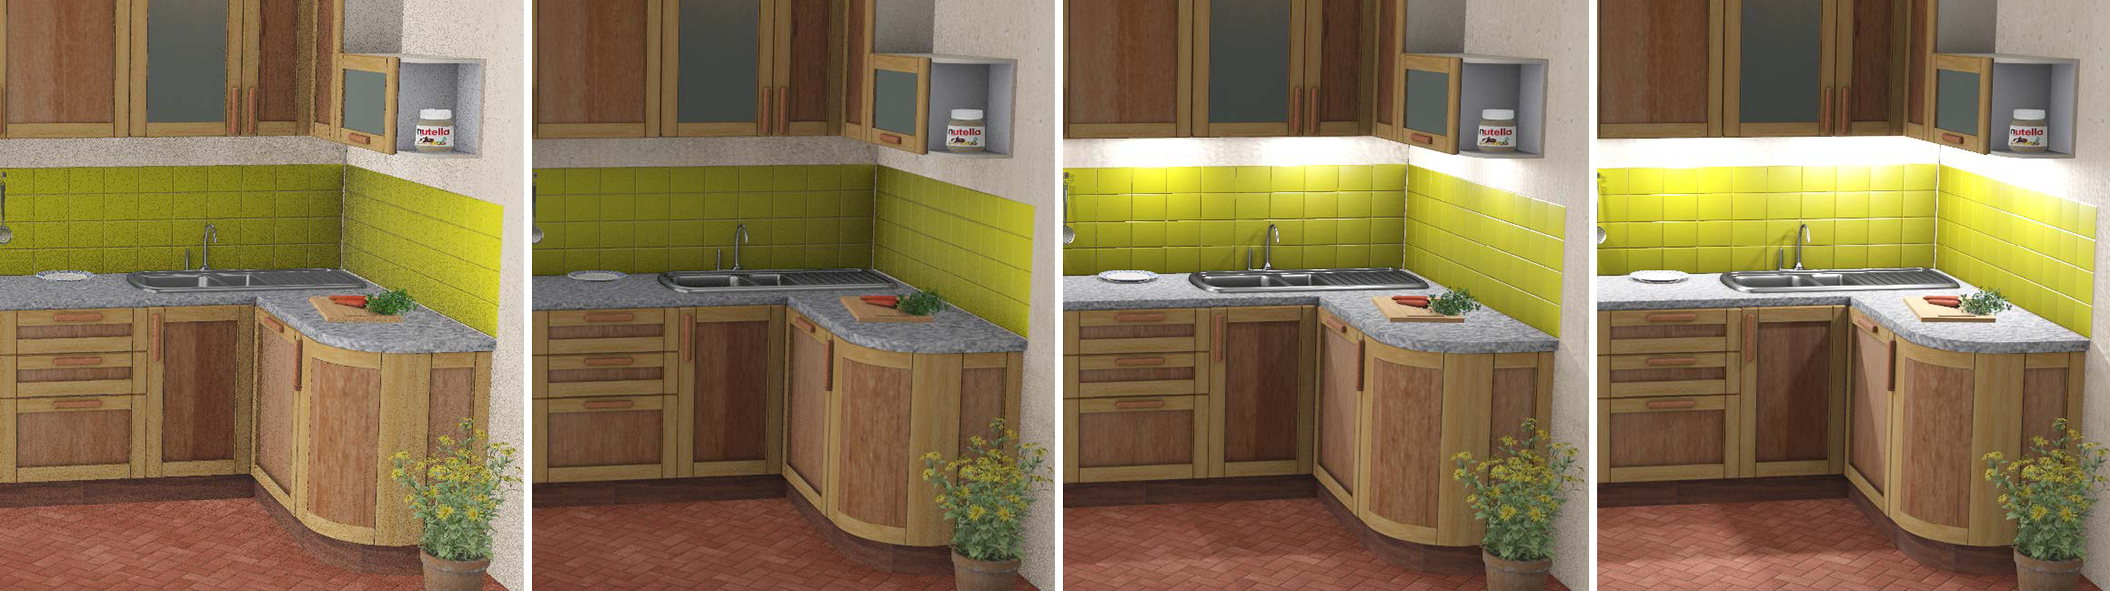
\includegraphics[trim=00 00 00 00, clip, width=\textwidth]{kitchen-ours-teaser-v2}
  \vspace{-2em}
  \caption{Intermediate frames of the kitchen model using our progressive renderer with a total frame count of 256 (right).}
  \vspace{+1em}
  \label{fig:teaser}
  \vspace{5mm}
\end{teaserfigure}

\maketitle

\vspace{5mm}
\section{Introduction}
\begin{figure*}
    \centering
    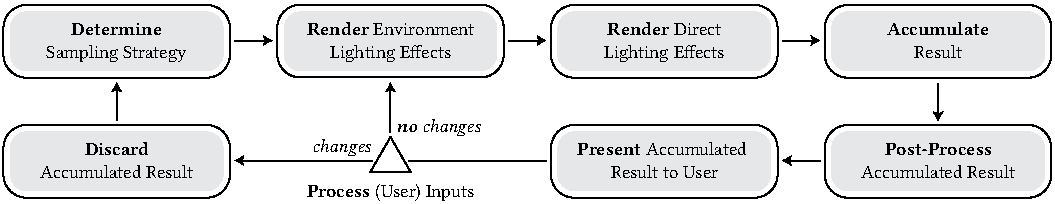
\includegraphics[width=\textwidth]{concept/webgl-progressive-light-pipeline}
    \caption{Workflow for progressive, physically-based rendering supporting environment and area lighting. }
    \label{fig:concept_workflow}
\end{figure*}

Using physically motivated rendering concepts is an important part of photo-realistic rendering.
These concepts incorporate physically-based reflection models, indirect lighting as well as the use of physical units for handling light intensity.
Due to the continuous increase in performance of rendering hardware, these concepts are considered for real-time rendering more and more.
We are now at a point, where mobile hardware is capable of running some of these physically motivated techniques.
In offline rendering, these concepts have been used for a long time~\cite{colbert2010importance}. 
In interactive real-time computer graphics applications, however, such techniques are prohibitively expensive.
As a result, approximations are used extensively in order to attain physically plausible results~\cite{karis2013real,lagarde2014moving}.

With a broad support for OpenGL ES 3.0 and WebGL 2.0~\cite{jackson2015webgl}, physically-based rendering has become feasible in the web and on mobile devices.
In comparison to desktop rendering, the support for physically-based concepts by many web rendering frameworks is still limited though.
The low performance of mobile graphics cards render most of the real-time approximations of today's game engines too expensive for use in the web.
In this work, we use progressive rendering~\cite{limberger2016progressive} for interactive, yet physically-based rendering in the web.
Progressive rendering distributes the rendering workload across multiple frames while showing intermediate results to the user.
It enables interactive and high quality rendering at the cost of temporal coherency and is mainly useful for static 3D geometry with no moving objects or lights.
We show how (1) area lights based on Karis' \cite{karis2013real} approach as well as (2) lighting by pre-filtered diffuse and specular cubemaps can be used in a progressive rendering setting.
In addition, we present a rendering technique for progressive computation of both diffuse and specular occlusion based on this pre-filtered environment lighting.
Besides our open source implementation, we provide a tool and discuss a tweak for pre-computation and storage of environment maps for image based lighting and web-based provisioning respectively.
Finally, we discuss strategies on workload distribution that allow smooth interaction on weaker hardware such as mobile devices.

A renderer capable of producing interactive, high-quality renderings of static scenes can be used for a number of web-based applications such as product configurators, online asset marketplaces or online modelling toolkits.
Additionally, a progressive renderer can be used to generate data sets for machine learning purposes.
This can be achieved by rendering the same scene with a high number of samples and a low number of samples.
The resulting images can then be used to train a network that is able to transform noisy images rendered at low sample counts to higher quality in real time.
Such an approach is used by \cite{chaitanya2017interactive} in order to reconstruct noisy images generated using Monte Carlo methods.

The goal of this work is to match the appearance of offline rendering results as closely as possible on mobile devices, while maintaining interactivity, e.g., for navigating the scene.
Therefore, we compare our results to both a rasterizer and a path tracer in regards to visual quality and rendering time.

\section{Related Work}
For related work, we discuss techniques of two areas, progressive rendering and physically-based rendering.

\paragraph{Progressive rendering}
Distributing samples of a rendering technique across multiple frames to enhance interactivity was first used by \cite{fuchs1985fast} to facilitate anti-aliasing.
This concept of \textit{progressive rendering} was extended by \cite{haeberli1990accumulation}, who introduced the \textit{accumulation buffer} in order to render effects such as anti-aliasing, soft shadows, and motion blur by rendering the same 3D geometry multiple times and accumulating the results of all intermediate frames.
In comparison to rendering the effects within one frame, intermediate results can be shown to the user, which allows smoother interaction with the scene.
\cite{limberger2016progressive} took this idea one step further and showed how to implement order-independent transparency, depth of field, screen-space ambient occlusion, soft-shadows and more.
This was later used to produce high-quality renderings of geo-referenced data~\cite{limberger2017cartography}.
\cite{sunet2016optimized} discuss approaches to optimize calculation of screen space ambient occlusion for mobile devices.
They suggest using progressive rendering in order to improve performance.
Multiple works on anti-aliasing are using temporal reprojection to use the results of the last frame for enhanced reconstruction,
e.g., SMAA \cite{jimenez2012smaa} and the Unreal Engine anti-aliasing implementation \cite{karis2014high}.
Temporal reprojection has been shown to work very well for low-frequency effects such as ambient occlusion and indirect lighting.
We decide against using it for our approach because for high-frequency direct lighting, the usual \enquote{ghosting} artifacts would be very noticeable.
Also it could lead to \enquote{half-lit} scenes during navigation when some parts of the image were successfully reprojected while others were not.

\paragraph{Physically-based rendering}
The microfacet model \cite{cook1982reflectance} was introduced as a way to model light reflection in a physically-based way.
\cite{walter2007microfacet} built on this concept and introduced a new distribution term, the GGX distribution.
For specular reflections, we use the Cook-Torrance model with the GGX distribution within our work.
Based on the microfacet mordel, \cite{burley2012physically} designed a BRDF model that uses the parameters \emph{roughness}, \emph{metallicness} and \emph{base color} to render a broad range of materials.
\cite{blinn1976texture} introduced a way of generating reflections of environment lighting on curved surfaces, based on texture mapping.
They store environment lighting data in textures and assume surfaces as perfect mirrors to obtain reflections.
\cite{greene1986environment} introduced the concept of the \textit{Cube Map} as a more efficient representation of environment light in textures.
Additionally, they describe how to filter cube maps based on the material properties and how to approximate this filtering process by pre-filtering the cube map via mip mapping.
This concept is used in our work to approximate environment lighting on surfaces with different material properties.
\cite{scheuermann2006cubemap} introduced the tool \textit{CubeMapGen}, which implements a pre-filtering of cubemaps for different BRDFs as described by Greene.
We implement a comparable tool (open source) that runs in the web to perform pre-processing of environment textures\footnote{\url{https://cgcostume.github.io/ermt/}}.
Karis \cite{karis2013real} introduce the \textit{split sum approximation} to approximate environment lighting using the GGX BRDF in a physically plausible way using only on environment map sample, which we use for the purpose of specular environment lighting.
Additionally, he shows an approach to approximate area lights using the GGX BRDF by considering a area lights as a point lights that are located as close to the reflection vector as possible.
With \textit{screen space ambient occlusion} (SSAO) \cite{mittring2007finding} an approach to render ambient occlusion as a post-processing effect was introduced.
\textit{Screen-space directional occlusion} \cite{ritschel2009approximating} improves on SSAO by considering the direction of occlusion and thus weights the environment lighting in a more physically correct way.
Additionally, one bounce of light is implemented by sampling the previous frame of the scene.
By generalizing screen-space occlusion for specular BRDFs, \cite{jimenez2016practical} describe a way to render specular occlusion in real-time.
We will show a technique to adapt these screen-space occlusion approaches to progressive rendering.
\cite{sturm2016unified} introduced extensions to glTF and X3D to support physically-based rendering using those formats.
These extensions have made their way into the glTF \cite{robinet2013gltf} standard, which we use for transmission and loading of 3D assets.
Applications of physically-based rendering in the web have been published as part of ThreeJS \footnote{\url{https://threejs.org/examples/webgl\_shading\_physical.html} and \url{https://threejs.org/examples/\#webgl\_lights\_rectarealight}}, as well as VirtualLightJS \footnote{\url{https://connect.unity.com/p/virtualightjs-webgl-pbr-engine}} by Guthmann François.
However, these demos show rather simple lighting scenarios and the shadowing is not physically modelled.
Also for VirtualLightJS aliasing artifacts are quite visible, which we want to overcome with our approach.

\section{Technique}
\begin{figure}
    \centering
    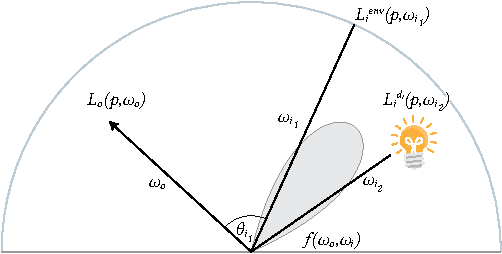
\includegraphics[width=\linewidth]{concept/webgl-progressive-light-concept}
    \caption{Illustration of outgoing radiance $L_o(p, \omega_o)$, incoming radiance from a distant environment $L_i^\text{env}(p, \omega_{i_1})$ and incoming direct lighting radiance $L_i^{d_i}(p, \omega_{i_2})$. Notice that $\omega_{i_1}$ and $\omega_{i_2}$ are only single solid angles out of the integral over the hemisphere $\Omega$.}
    \label{fig:rendering_variables}
\end{figure} 

For our progressive rendering approach we propose a workflow that, prior to the synthesis of intermediate frames, determines a sampling strategy for rendering lighting effects. 
For each intermediate frame, environment lighting effects and direct lighting effects are then evaluated independently from one another.
The results of these calculations are then accumulated with the results of previous intermediate frames, a common operation in progressive renderers.
After a post-processing step is applied, the result is presented to the user, before continuing with the next intermediate frame and starting this process again.
This process is depicted in Figure~\ref{fig:concept_workflow}.

To calculate the radiance emitted from a point $p$ within a 3D scene, Pharr et al. \cite{pharr2016physically} give:
\begin{align}
    L_o(p, \omega_o) &= \int_\Omega f(\omega_o, \omega_i) L_i(p, \omega_i) \left|\cos \theta_i\right| d\omega_i,
\end{align}
where $\Omega$ is the hemisphere around the point $p$, $\omega_o$ is the direction of the outgoing radiance, $f$ is the \emph{bidirectional reflectance distribution function} (BRDF), $L_i$ is the incoming radiance from a direction $\omega_i$ and $\theta_i$ is the angle between incoming and outgoing light directions.
To approximate this equation, we will model direct lighting by light sources and lighting caused by environment effects separately:
\begin{align}
    L_o(p, \omega_o) &\approx L_o^\text{env}(p, \omega_o) + \sum_{i = 1}^n L_o^{d_i}(p, \omega_o), \label{math:lighting_approx}
\end{align}
where $L_o^\text{env}(p, \omega_o)$ is the radiance emitted from $p$ due to lighting from a distant environment and $L_o^{d_i}(p, \omega_o)$ is the radiance emitted from $p$ due to emission from the area light source with index $i$ (Figure~\ref{fig:rendering_variables}).
Even though Equation \ref{math:lighting_approx} is an approximation, $L_o^\text{env}(p, \omega_o)$ and $L_o^{d_i}(p, \omega_o)$ are still integrals for which accurate evaluation is not feasible.
Therefore, we discuss approximations of these terms using progressive rendering in the following subsections.
We model the reflection of surfaces using two separate BRDFs.
For the diffuse case, we assume lambertian reflection $f(\omega_o, \omega_k) = \frac{c}{\pi}$, where $c$ is the diffuse color of the material.
For specular reflections, we use the Cook-Torrance model with the GGX distribution term.
The result of applying these BRDFs in a sample scene can be seen in Figure \ref{fig:brdf_comparison}.

\begin{figure}
    \centering

    \begin{subfigure}[b]{0.325\columnwidth}
        \begin{tikzpicture}[spy using outlines={white, circle, magnification=2.5, size=40, connect spies, every spy on node/.append style={thin}}]
            \node[anchor=center, inner sep=0pt, outer sep=0pt](initial) {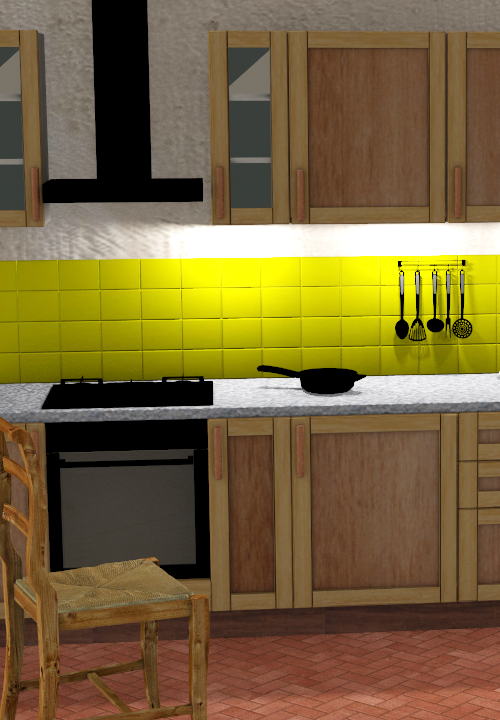
\includegraphics[width=\textwidth]{concept/brdfs/kitchen_diffonly.png}};%
            \spy on ($(initial)+(1.0, +0.3)$) in node at (-0.5, 1.1);
        \end{tikzpicture}
        \caption{Diffuse}
    \end{subfigure}
    \begin{subfigure}[b]{0.325\columnwidth}
        \begin{tikzpicture}[spy using outlines={white, circle, magnification=2.5, size=40, connect spies, every spy on node/.append style={thin}}]
            \node[anchor=center, inner sep=0pt, outer sep=0pt](initial) {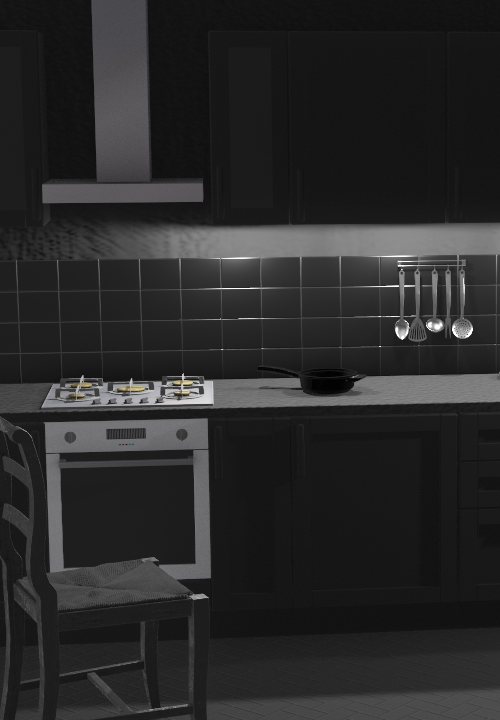
\includegraphics[width=\textwidth]{concept/brdfs/kitchen_speconly.png}};%
            \spy on ($(initial)+(1.0, +0.3)$) in node at (-0.5, 1.1);
        \end{tikzpicture}
        \caption{Specular}
    \end{subfigure}
    \begin{subfigure}[b]{0.325\columnwidth}
        \begin{tikzpicture}[spy using outlines={white, circle, magnification=2.5, size=40, connect spies, every spy on node/.append style={thin}}]
            \node[anchor=center, inner sep=0pt, outer sep=0pt](initial) {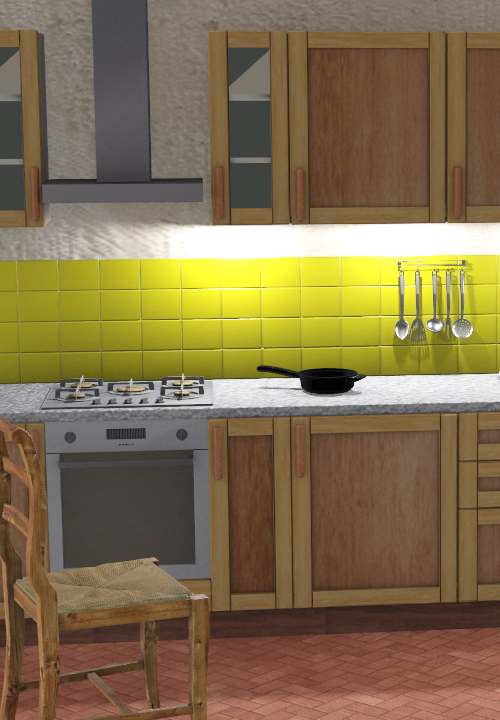
\includegraphics[width=\textwidth]{concept/brdfs/kitchen_full.png}};%
            \spy on ($(initial)+(1.0, +0.3)$) in node at (-0.5, 1.1);
        \end{tikzpicture}
        \caption{Combined}
    \end{subfigure}
    \vspace{-1.2em}
    \caption{Visualization of the diffuse and specular lighting components of a rendering of a kitchen.}
    \label{fig:brdf_comparison}
\end{figure}

\subsection{Rendering Environment Lighting Effects}
In order to render environment reflections fast, we pre-filter the environment textures both the diffuse and specular BRDF.
Since lambertian reflection is not view dependent, it can be accurately pre-calculated ahead of rendering time by using Monte Carlo integration.
At rendering time, the pre-filtered environment map is then sampled using the normal vector to get an approximation of the diffuse environment lighting.
\begin{figure}
    \centering
       
    \begin{subfigure}[b]{0.24\columnwidth}
        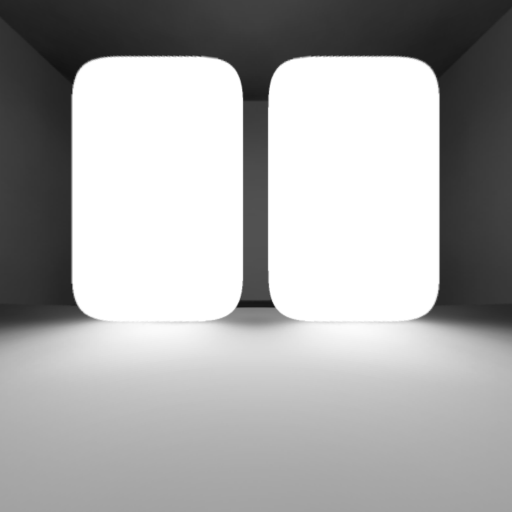
\includegraphics[width=\columnwidth]{concept/prefiltering/preprocessed-map-nx-0.png}
        \caption{512x512}
    \end{subfigure}
    \begin{subfigure}[b]{0.24\columnwidth}
        
\includegraphics[width=\columnwidth]{concept/prefiltering/preprocessed-map-nx-1.png}
        \caption{256x256}
    \end{subfigure}
    \begin{subfigure}[b]{0.24\columnwidth}
        
\includegraphics[width=\columnwidth]{concept/prefiltering/preprocessed-map-nx-2.png}
        \caption{128x128}
    \end{subfigure}
    \begin{subfigure}[b]{0.24\columnwidth}
        
\includegraphics[width=\columnwidth]{concept/prefiltering/preprocessed-map-nx-3.png}
        \caption{64x64}
    \end{subfigure}
    
    \begin{subfigure}[b]{0.24\columnwidth}
        
\includegraphics[width=\columnwidth]{concept/prefiltering/preprocessed-map-nx-4.png}
        \caption{32x32}
    \end{subfigure}
    \begin{subfigure}[b]{0.24\columnwidth}
        
\includegraphics[width=\columnwidth]{concept/prefiltering/preprocessed-map-nx-5.png}
        \caption{16x16}
    \end{subfigure}
    \begin{subfigure}[b]{0.24\columnwidth}
        
\includegraphics[width=\columnwidth]{concept/prefiltering/preprocessed-map-nx-6.png}
        \caption{8x8}
    \end{subfigure}
    \begin{subfigure}[b]{0.24\columnwidth}
        
\includegraphics[width=\columnwidth]{concept/prefiltering/preprocessed-map-nx-7.png}
        \caption{4x4}
    \end{subfigure}
    
    \vspace{-1.2em}
    \caption{Mipmap levels of a face of a pre-filtered specular environment map using the GGX distribution. The images were created with our web-based tool, taking an equirectangular map as input and outputing 6 face of a cube map.}
    \label{fig:prefiltered_environment}
\end{figure}
For specular reflections, we use the GGX BRDF, which is view dependent, making accurate pre-filtering impossible.
We use Karis' \textit{split sum approximation}~\cite{karis2013real} to still get physically plausible results using pre-filtering.
Karis approximates Monte Carlo integration in the following way:
\begin{align}
    L_o^\text{env}(p, \omega_o) &\approx \frac{1}{n} \sum_{k = 1}^n \frac{f(\omega_o, \omega_k) L_i^\text{env}(p, \omega_k) \left|\cos \theta_k\right|}{q(\omega_o, \omega_k)}\\
    &\approx \left(\frac{1}{n} \sum_{k = 1}^n L_i^\text{env}(p, \omega_k) \right) \left( \frac{1}{n} \sum_{k = 1}^n \frac{f(\omega_o, \omega_k) \left|\cos \theta_k\right|}{q(\omega_o, \omega_k)} \right). \label{math:split_sum}
\end{align}
Since the left sum is now independent of $\omega_o$, i.e., it is not view-dependent, it can easily be pre-calculated.
To enable an efficient lookup at render time, multiple resolutions are pre-calculated based different roughness values and stored in the mipmap chain of the environment texture (Figure~\ref{fig:prefiltered_environment}).
The second sum represents all other factors as if they were integrated against a fully white environment.
It dependents on a materials roughness and $\left|\cos \theta_k\right|$.
Therefore we pre-calculate it as a 2D texture lookup of these two values.
\begin{figure}[b]
    \centering
    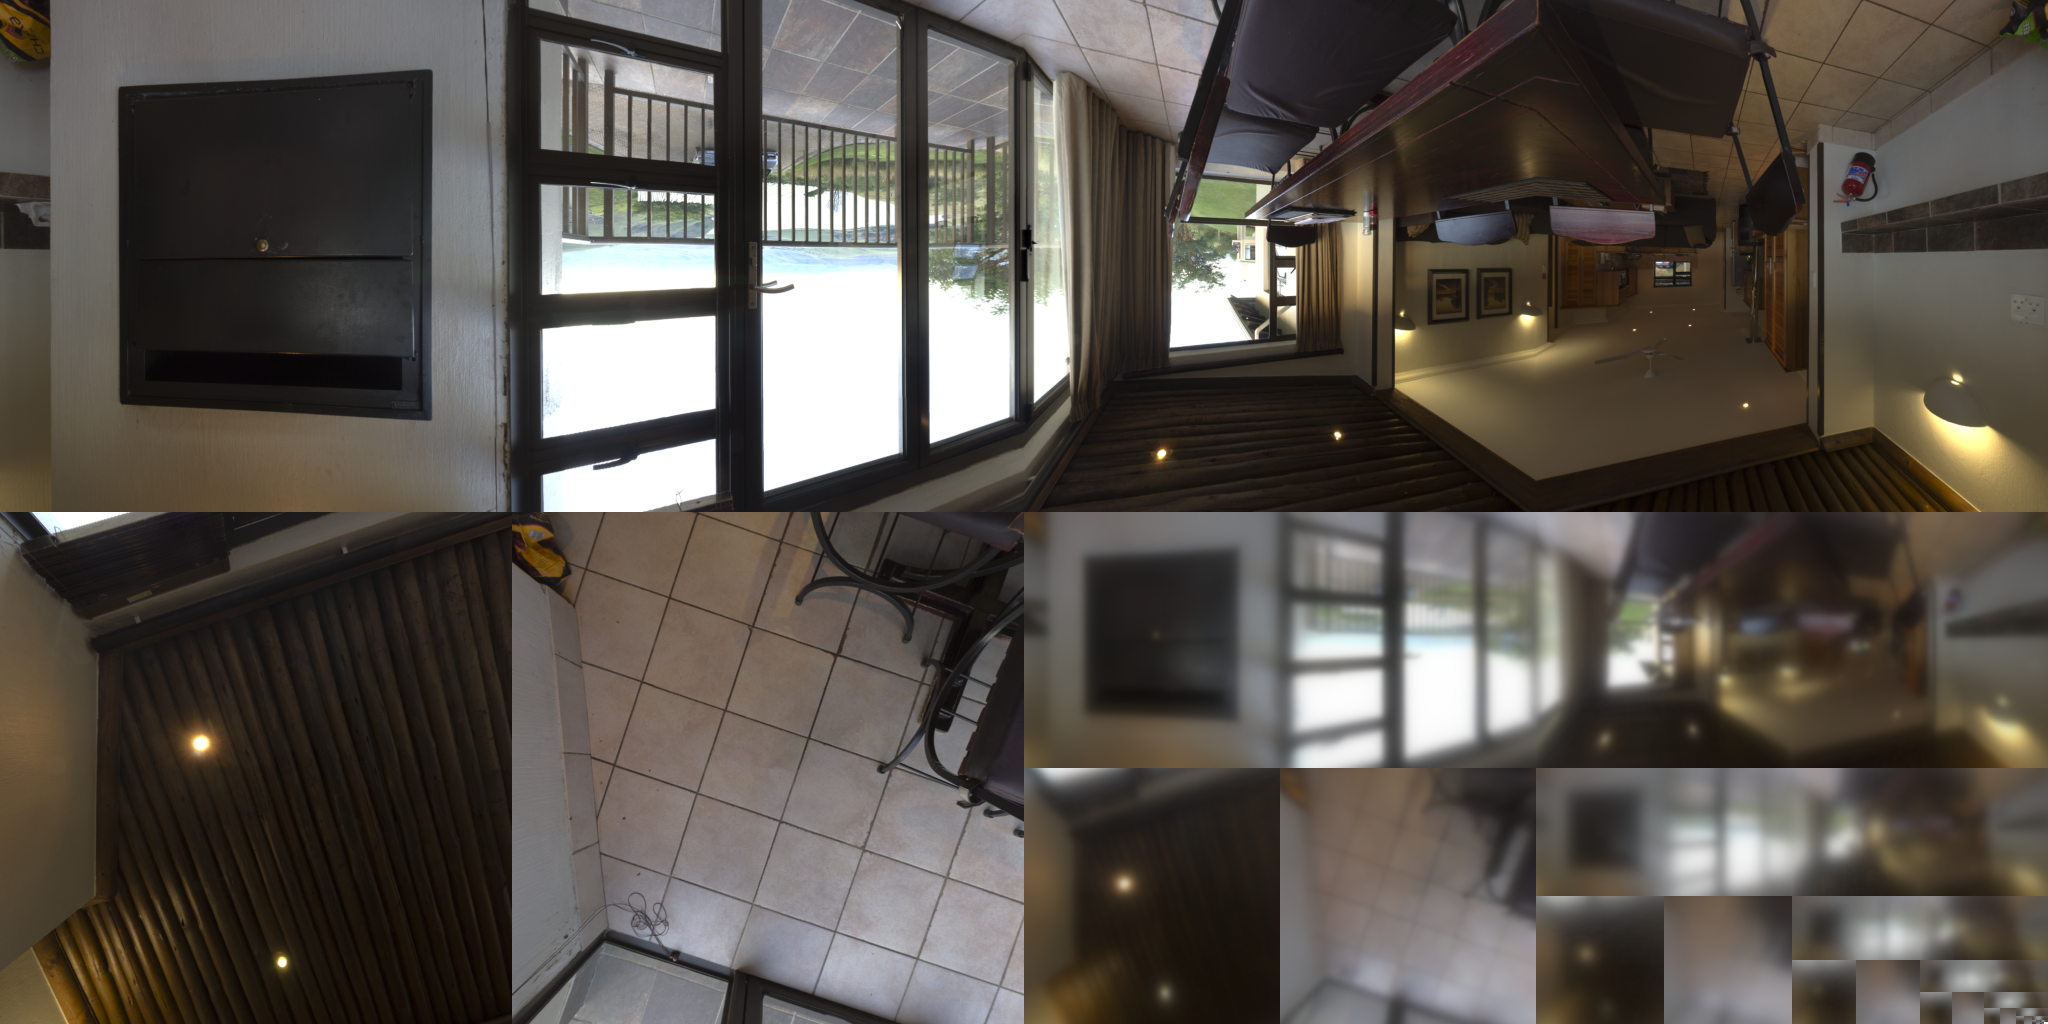
\includegraphics[width=\columnwidth]{concept/prefiltering/ibl-map}
    \vspace*{-1.2em}
    \caption{Efficient storage of all cube map faces of all mipmap levels within a single texture. 
    This reduces the number of requests significantly while slightly increasing the complexity of loading individual faces. 
    Input image---an equirectangular foto---taken from \href{https://hdrihaven.com}{hdrihaven.com}.}
    \label{fig:concept_storage}
\end{figure}
At render time the pre-filtered environment map is sampled using the reflection vector.
The appropriate mipmap level is calculated based on the material's roughness.
The other sum is sampled from the lookup texture using roughness and $\left|\cos \theta_k\right|$ as texture coordinates.

\subsection{Diffuse and Specular Occlusion}
\label{subsec:occlusion}
\begin{figure}
    \centering
    
    \begin{subfigure}[b]{0.24\columnwidth}
        \begin{tikzpicture}[spy using outlines={gray, circle, magnification=2, size=60, connect spies, every spy on node/.append style={thin}}]
            \node[anchor=center, inner sep=0pt, outer sep=0pt](initial) {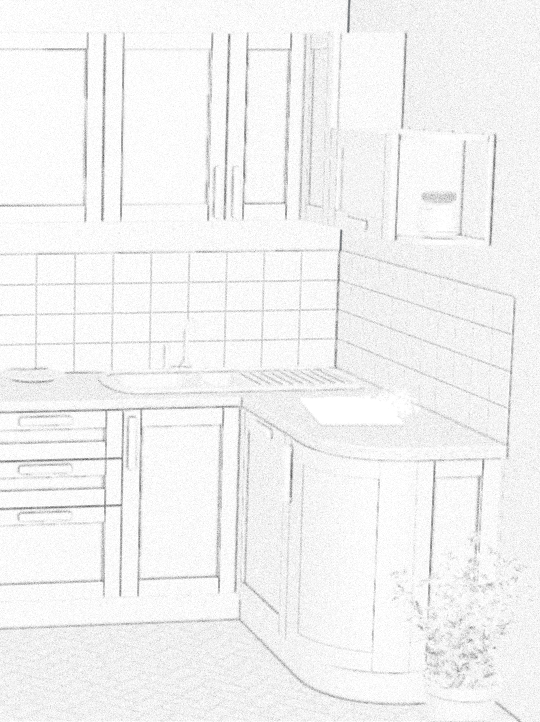
\includegraphics[width=\textwidth]{concept/diffuse_occlusion/kitchen_occlusion005.png}};%
        \end{tikzpicture}
        \caption{$d_\text{occ} = 0.05$}
    \end{subfigure}
    \begin{subfigure}[b]{0.24\columnwidth}
        \begin{tikzpicture}[spy using outlines={gray, circle, magnification=2, size=60, connect spies, every spy on node/.append style={thin}}]
            \node[anchor=center, inner sep=0pt, outer sep=0pt](initial) {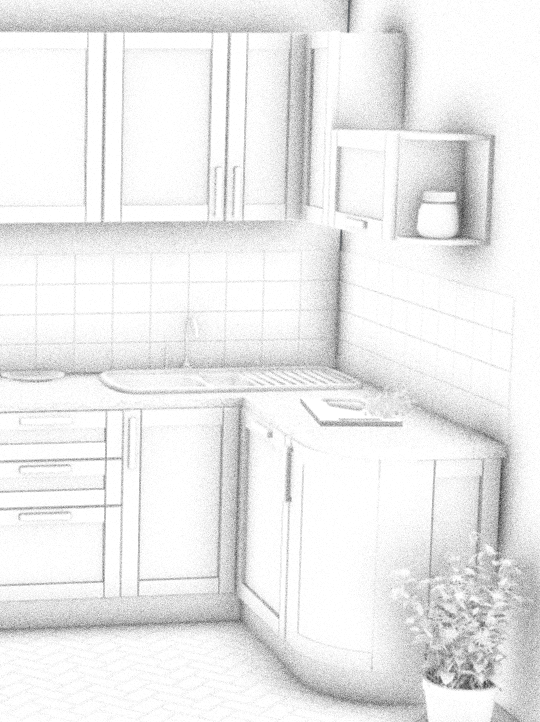
\includegraphics[width=\textwidth]{concept/diffuse_occlusion/kitchen_occlusion025.png}};%
        \end{tikzpicture}
        \caption{$d_\text{occ} = 0.25$}
    \end{subfigure}
    \begin{subfigure}[b]{0.24\columnwidth}
        \begin{tikzpicture}[spy using outlines={gray, circle, magnification=2, size=60, connect spies, every spy on node/.append style={thin}}]
            \node[anchor=center, inner sep=0pt, outer sep=0pt](initial) {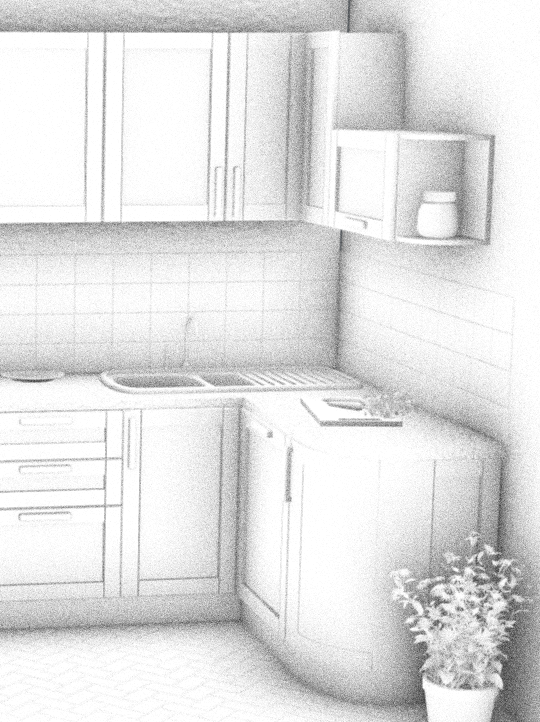
\includegraphics[width=\textwidth]{concept/diffuse_occlusion/kitchen_occlusion050.png}};%
        \end{tikzpicture}
        \caption{$d_\text{occ} = 0.5$}
    \end{subfigure}
    \begin{subfigure}[b]{0.24\columnwidth}
        \begin{tikzpicture}[spy using outlines={gray, circle, magnification=2, size=60, connect spies, every spy on node/.append style={thin}}]
            \node[anchor=center, inner sep=0pt, outer sep=0pt](initial) {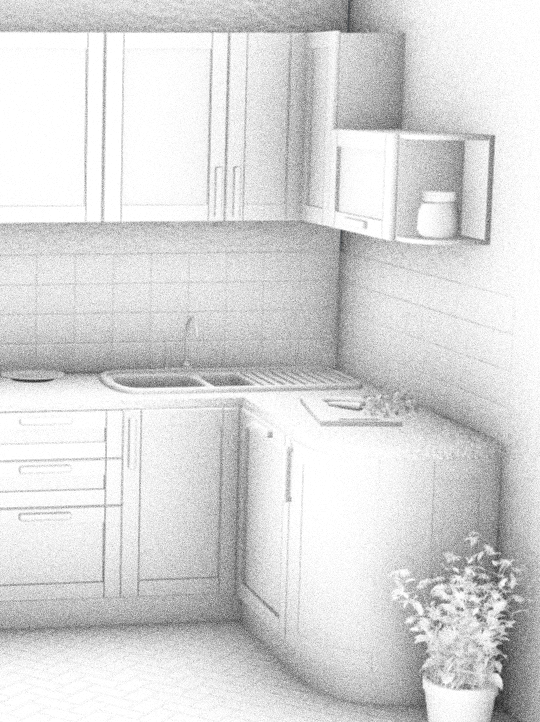
\includegraphics[width=\textwidth]{concept/diffuse_occlusion/kitchen_occlusion075.png}};%
        \end{tikzpicture}
        \caption{$d_\text{occ} = 0.75$}
    \end{subfigure}
    
    \begin{subfigure}[b]{0.24\columnwidth}
        \begin{tikzpicture}[spy using outlines={gray, circle, magnification=2, size=60, connect spies, every spy on node/.append style={thin}}]
            \node[anchor=center, inner sep=0pt, outer sep=0pt](initial) {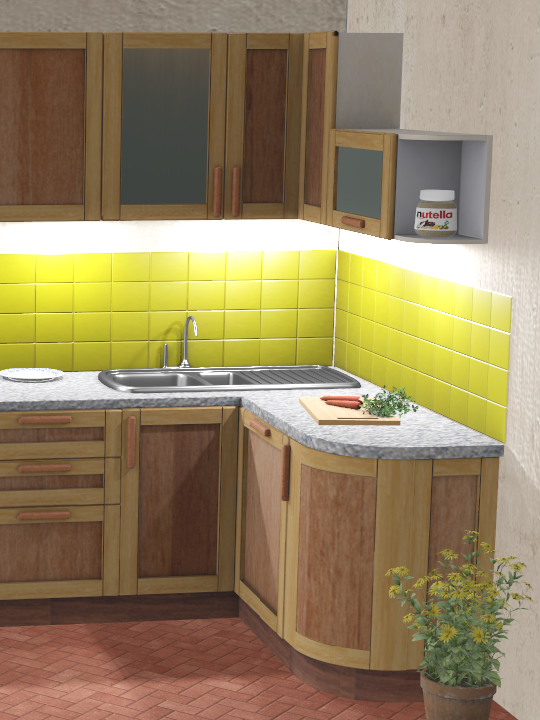
\includegraphics[width=\textwidth]{concept/diffuse_occlusion/kitchen_lit_noocclusion_256samples.png}};%
        \end{tikzpicture}
        \caption{None}
    \end{subfigure}
    \begin{subfigure}[b]{0.24\columnwidth}
        \begin{tikzpicture}[spy using outlines={gray, circle, magnification=2, size=60, connect spies, every spy on node/.append style={thin}}]
            \node[anchor=center, inner sep=0pt, outer sep=0pt](initial) {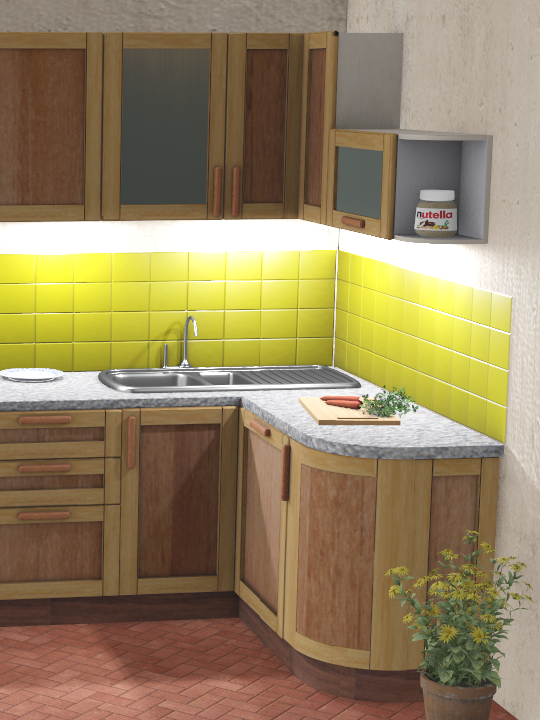
\includegraphics[width=\textwidth]{concept/diffuse_occlusion/kitchen_lit_occlusion025_256samples.png}};%
        \end{tikzpicture}
        \caption{$d_\text{occ} = 0.25$}
    \end{subfigure}
    \begin{subfigure}[b]{0.24\columnwidth}
        \begin{tikzpicture}[spy using outlines={gray, circle, magnification=2, size=60, connect spies, every spy on node/.append style={thin}}]
            \node[anchor=center, inner sep=0pt, outer sep=0pt](initial) {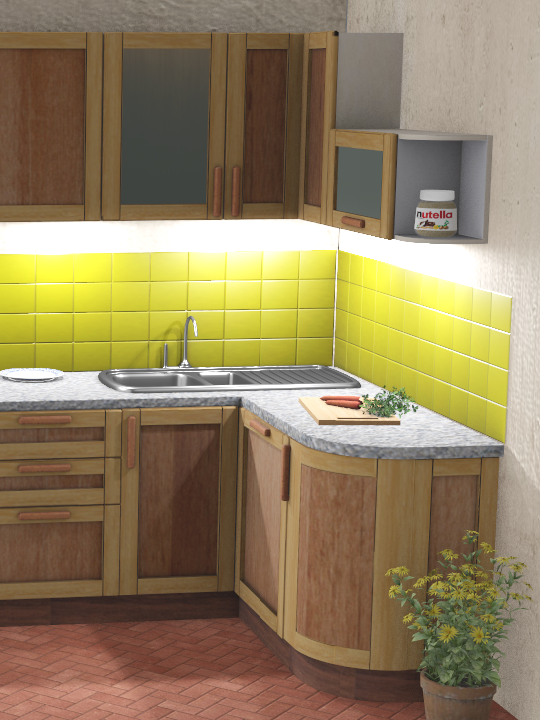
\includegraphics[width=\textwidth]{concept/diffuse_occlusion/kitchen_lit_occlusion050_256samples.png}};%
        \end{tikzpicture}
        \caption{$d_\text{occ} = 0.5$}
    \end{subfigure}
    \begin{subfigure}[b]{0.24\columnwidth}
        \begin{tikzpicture}[spy using outlines={gray, circle, magnification=2, size=60, connect spies, every spy on node/.append style={thin}}]
            \node[anchor=center, inner sep=0pt, outer sep=0pt](initial) {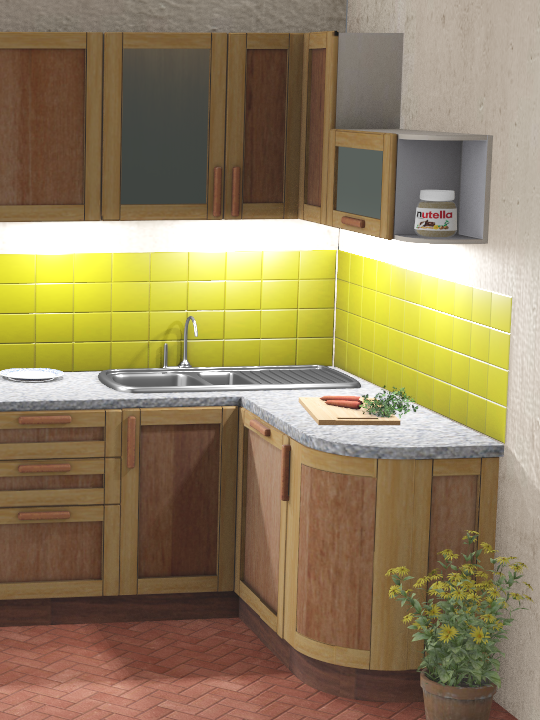
\includegraphics[width=\textwidth]{concept/diffuse_occlusion/kitchen_lit_occlusion075_256samples.png}};%
        \end{tikzpicture}
        \caption{$d_\text{occ} = 0.75$}
    \end{subfigure}
    
    \vspace{-1.2em}
    \caption{Rendering result of different occlusion distances $d_\text{occ}$. Top row: areas that are affected by diffuse occlusion are displayed dark, bottom row: rendering result. Note that the occlusion is less visible in the final rendering because it only affects environment lighting and not direct lighting.}
    \label{fig:diffuse_occlusion_rendering}
\end{figure}

Using pre-filtered lookups from environment textures allows us to approximate environment lighting.
However, this does not account for occlusion by nearby objects within the scene.
Calculating physically correct occlusion is hard to achieve in real-time rendering and commonly approximated using \textit{screen-space ambient occlusion} which darkens ambient lighting based on blockers in screen-space.
We adapt this technique for use in a progressive rendering and, additionally, apply a similar technique to determine specular occlusion as well.
We assume that depth and normal buffers of the rendered scene are available while rendering the scene.
It is often sufficient to generate them only once with each camera change.

Let $d_i$ and $s_i$ be sets of diffuse and specular samples that are calculated during frame number $i$.
For each sample, a tangent space vector is generated using importance sampling using the corresponding BRDF of the sample.
For diffuse samples, a cosine weighted sample within the hemisphere is generated and transformed to a view space vector $v$.
For specular samples, a half-vector is generated according to the material properties of the rendered surface and the reflection of the view vector at this half-vector is calculated to get the view space vector $v$.
$v$ determines the direction in which the occlusion is evaluated for this sample.
It is scaled by the occlusion distance $d_\text{occ}$.
Using this scaled vector, we calculate the sampling point $p = s + v$, where $s$ is the view-space position of the shaded point.
Let $d_p$ be the view-space depth of $p$.
$p$ is transformed to normalized device coordinates and used to sample the screen-space depth $d_s$ from the scene depth texture.
Now, if $d_p > d_s$ the evaluated sample is considered to be occluding.
Therefore, environment lighting from the sampled BRDF will not be added to the total scene lighting, which darkens the occluded area.
The effect of diffuse and specular occlusion can be seen in Figures \ref{fig:diffuse_occlusion_rendering} and \ref{fig:specular_occlusion_rendering}.

\begin{figure}
    \centering
    
    \begin{subfigure}[b]{0.24\columnwidth}
        \begin{tikzpicture}[spy using outlines={black, circle, magnification=2.5, size=40, connect spies, every spy on node/.append style={thin}}, inner sep=0pt, outer sep=0pt]
            \node[anchor=center, inner sep=0pt, outer sep=0pt](initial) {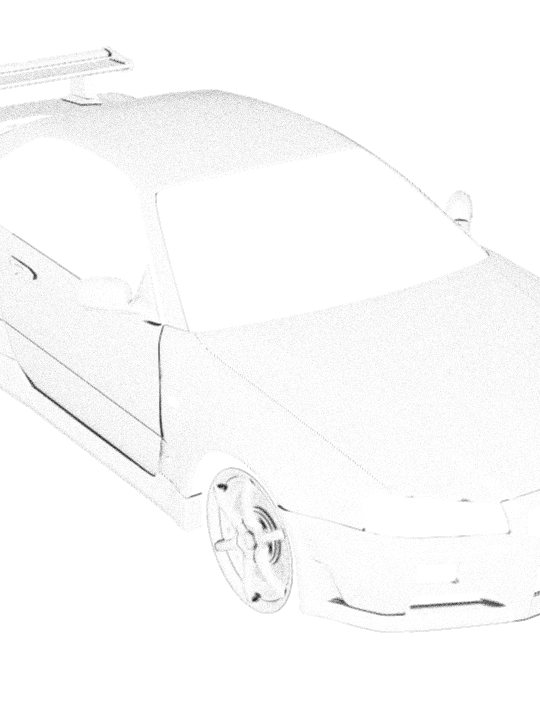
\includegraphics[width=\textwidth]{concept/specular_occlusion/skyline_occlusion005.png}};%
            \spy on ($(initial)+(-0.1, -0.6)$) in node at (0.5, 0.8);
        \end{tikzpicture}
        \caption{$d_\text{occ} = 0.05$}
    \end{subfigure}
    \begin{subfigure}[b]{0.24\columnwidth}
        \begin{tikzpicture}[spy using outlines={black, circle, magnification=2.5, size=40, connect spies, every spy on node/.append style={thin}}, inner sep=0pt, outer sep=0pt]
            \node[anchor=center, inner sep=0pt, outer sep=0pt](initial) {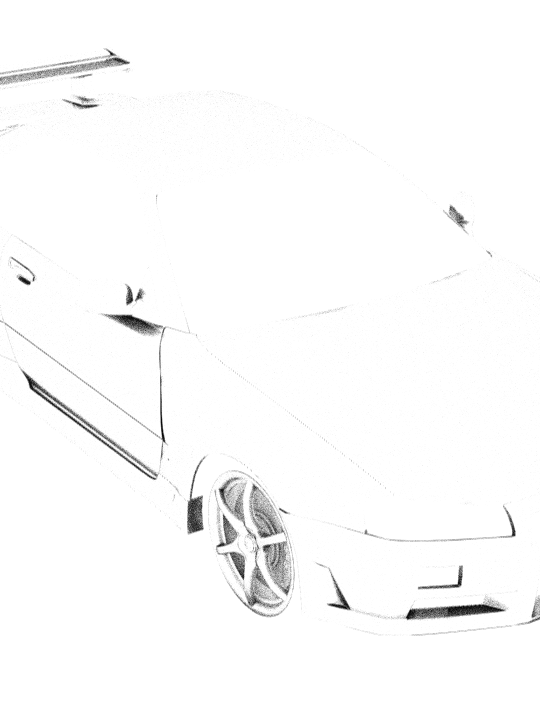
\includegraphics[width=\textwidth]{concept/specular_occlusion/skyline_occlusion025.png}};%
            \spy on ($(initial)+(-0.1, -0.6)$) in node at (0.5, 0.8);
        \end{tikzpicture}
        \caption{$d_\text{occ} = 0.25$}
    \end{subfigure}
    \begin{subfigure}[b]{0.24\columnwidth}
        \begin{tikzpicture}[spy using outlines={black, circle, magnification=2.5, size=40, connect spies, every spy on node/.append style={thin}}, inner sep=0pt, outer sep=0pt]
            \node[anchor=center, inner sep=0pt, outer sep=0pt](initial) {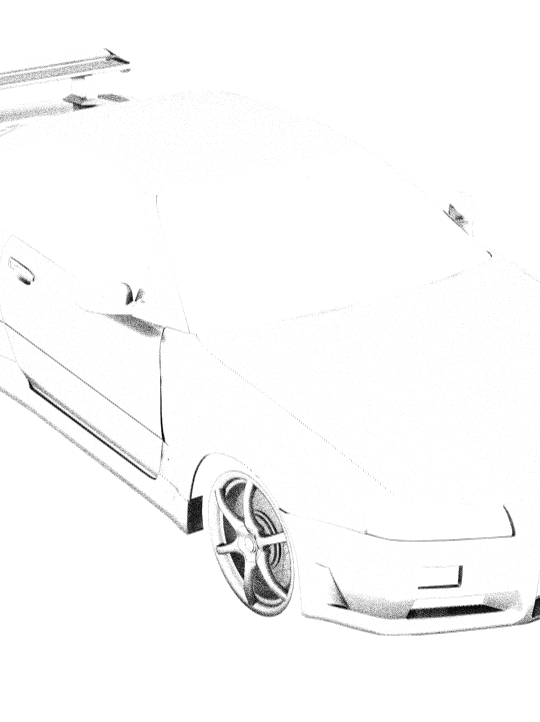
\includegraphics[width=\textwidth]{concept/specular_occlusion/skyline_occlusion050.png}};%
            \spy on ($(initial)+(-0.1, -0.6)$) in node at (0.5, 0.8);
        \end{tikzpicture}
        \caption{$d_\text{occ} = 0.5$}
    \end{subfigure}
    \begin{subfigure}[b]{0.24\columnwidth}
        \begin{tikzpicture}[spy using outlines={black, circle, magnification=2.5, size=40, connect spies, every spy on node/.append style={thin}}, inner sep=0pt, outer sep=0pt]
            \node[anchor=center, inner sep=0pt, outer sep=0pt](initial) {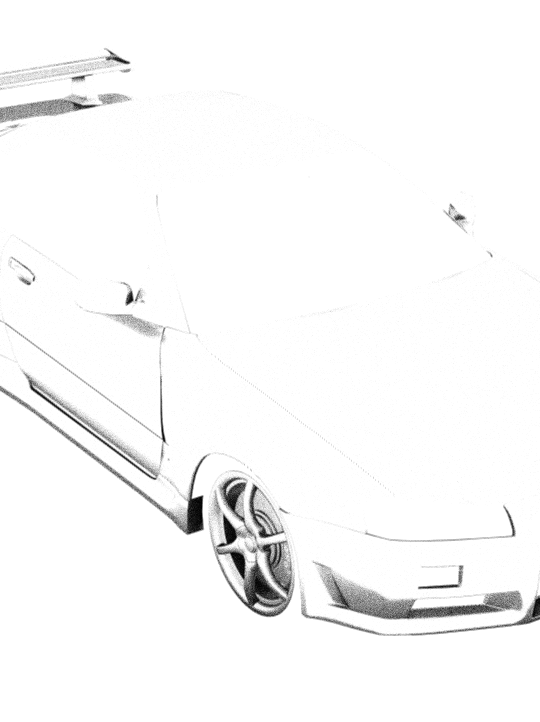
\includegraphics[width=\textwidth]{concept/specular_occlusion/skyline_occlusion075.png}};%
            \spy on ($(initial)+(-0.1, -0.6)$) in node at (0.5, 0.8);
        \end{tikzpicture}
        \caption{$d_\text{occ} = 0.75$}
    \end{subfigure}
    
    \begin{subfigure}[b]{0.24\columnwidth}
        \begin{tikzpicture}[spy using outlines={white, circle, magnification=2.5, size=40, connect spies, every spy on node/.append style={thin}}, inner sep=0pt, outer sep=0pt]
            \node[anchor=center, inner sep=0pt, outer sep=0pt](initial) {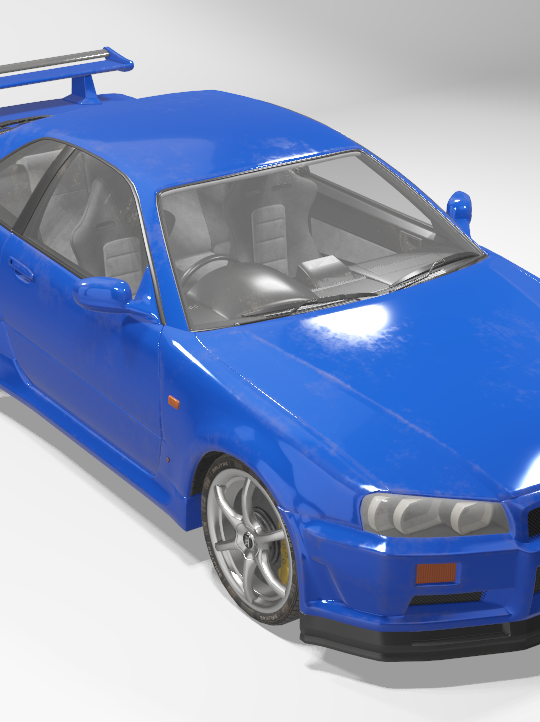
\includegraphics[width=\textwidth]{concept/specular_occlusion/skyline_lit_noocclusion.png}};%
            \spy on ($(initial)+(-0.1, -0.6)$) in node at (0.5, 0.8);
        \end{tikzpicture}
        \caption{None}
    \end{subfigure}
    \begin{subfigure}[b]{0.24\columnwidth}
        \begin{tikzpicture}[spy using outlines={white, circle, magnification=2.5, size=40, connect spies, every spy on node/.append style={thin}}, inner sep=0pt, outer sep=0pt]
            \node[anchor=center, inner sep=0pt, outer sep=0pt](initial) {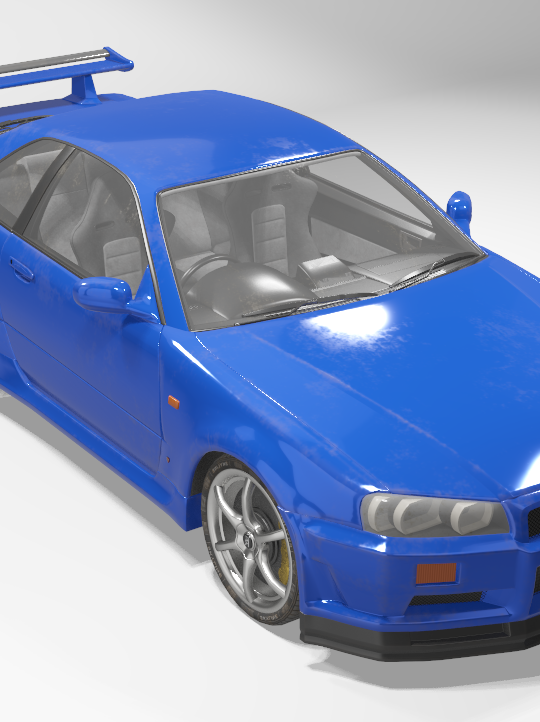
\includegraphics[width=\textwidth]{concept/specular_occlusion/skyline_lit025.png}};%
            \spy on ($(initial)+(-0.1, -0.6)$) in node at (0.5, 0.8);
        \end{tikzpicture}
        \caption{$d_\text{occ} = 0.25$}
    \end{subfigure}
    \begin{subfigure}[b]{0.24\columnwidth}
        \begin{tikzpicture}[spy using outlines={white, circle, magnification=2.5, size=40, connect spies, every spy on node/.append style={thin}}, inner sep=0pt, outer sep=0pt]
            \node[anchor=center, inner sep=0pt, outer sep=0pt](initial) {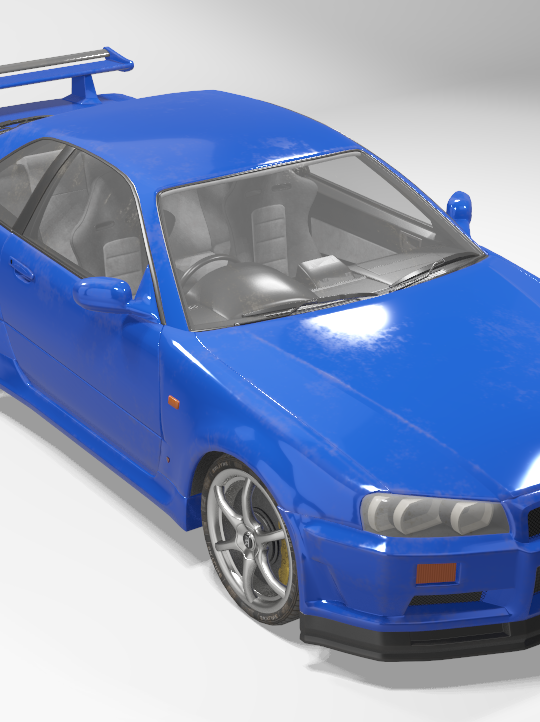
\includegraphics[width=\textwidth]{concept/specular_occlusion/skyline_lit050.png}};%
            \spy on ($(initial)+(-0.1, -0.6)$) in node at (0.5, 0.8);
        \end{tikzpicture}
        \caption{$d_\text{occ} = 0.5$}
    \end{subfigure}
    \begin{subfigure}[b]{0.24\columnwidth}
        \begin{tikzpicture}[spy using outlines={white, circle, magnification=2.5, size=40, connect spies, every spy on node/.append style={thin}}, inner sep=0pt, outer sep=0pt]
            \node[anchor=center, inner sep=0pt, outer sep=0pt](initial) {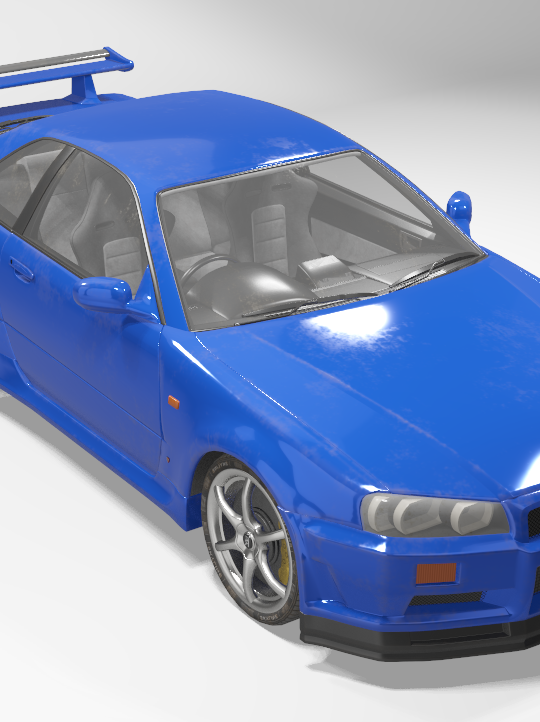
\includegraphics[width=\textwidth]{concept/specular_occlusion/skyline_lit075.png}};%
            \spy on ($(initial)+(-0.1, -0.6)$) in node at (0.5, 0.8);
        \end{tikzpicture}
        \caption{$d_\text{occ} = 0.75$}
    \end{subfigure}

    \vspace{-1.2em}
    \caption{Rendering result of different occlusion distances $d_\text{occ}$. Notice that only metallic surfaces are affected by specular occlusion. Top row: areas that are affected by specular occlusion are displayed dark, bottom row: rendering result.}
    \label{fig:specular_occlusion_rendering}
\end{figure}

\subsection{Progressive Area lighting}
To calculate the radiance produced by an area light we have
\begin{align}
    L_o^{d_i}(p, \omega_o) &= \int_{A_i} f(\omega_o, \omega_i) L_i^{d_i}(p, \omega_i) \left|\cos \theta_i\right| \frac{\cos \theta_o}{r^2} dA_i,
\end{align}
where we assume the outgoing radiance from a light source $L_i^{d_i}(p, \omega_i)$ to be constant, i.e., we model lights that have constant intensity across the whole area.
In the context of a progressive rendering system, we can use a few samples per light source, but we are still quite limited in resources.
Therefore, to calculate the intensity of specular reflections of area light sources we use Karis' \cite{karis2013real} approximation of the \textit{most representative point}:
\begin{align}
    L_o^{d_i}(p, \omega_o) &\approx f(\omega_o, \omega_r) E_A(p) \left|\cos \theta_i\right|,
\end{align}
where $\omega_r$ is the direction pointing to the most representative point and $E_A(p)$ is the irradiance arriving at point $p$ from area light source $A$.
The approximation for this most representative point is the point on the area light source, which is closest to the reflection of the view vector about the normal vector.
We can now approximate $E_A(p)$ by assuming $A$ is a point light source located at the most representative point:
\begin{align}
    E_A(p) &= \int_\Omega L_i^{d_i}(p, \omega_i) \left|\cos \theta_i\right| d\omega_i\\
    &\approx \frac{\phi_A}{4 \pi d^2},
\end{align}
where $\phi_A$ is the total power of the area light source.
Combining these equations we get
\begin{align}
    L_o^{d_i}(p, \omega_o) &\approx f(\omega_o, \omega_r) \frac{\phi_A}{4 \pi d^2} \left|\cos \theta_i\right| \label{math:direct_light_approx}.
\end{align}

\begin{figure}
    \centering
    \begin{subfigure}[b]{0.325\columnwidth}
        \begin{tikzpicture}[spy using outlines={white, circle, magnification=4, size=40, connect spies, every spy on node/.append style={thin}}]
            \node[anchor=center, inner sep=0pt, outer sep=0pt](initial) {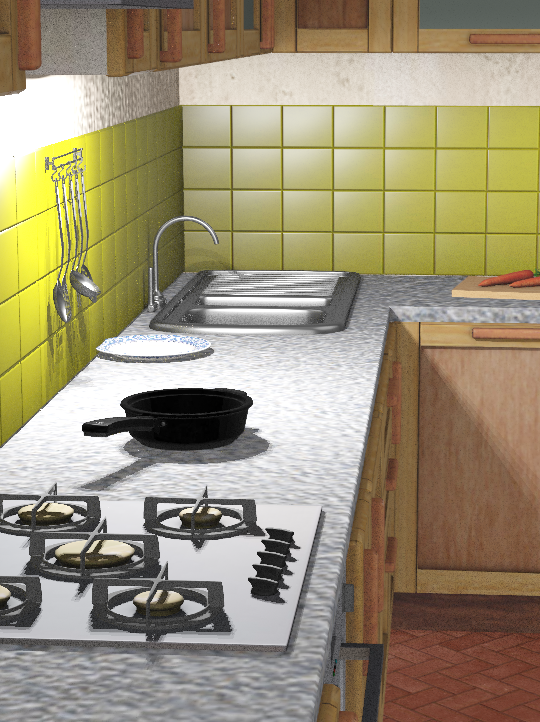
\includegraphics[width=\textwidth]{concept/area_light/kitchen_light_4samples.png}};%
            \spy on ($(initial)+(1.05, -0.3)$) in node at (-0.2, 0.9);
        \end{tikzpicture}
        \caption{4 samples}
    \end{subfigure}
    \begin{subfigure}[b]{0.325\columnwidth}
        \begin{tikzpicture}[spy using outlines={white, circle, magnification=4, size=40, connect spies, every spy on node/.append style={thin}}]
            \node[anchor=center, inner sep=0pt, outer sep=0pt](initial) {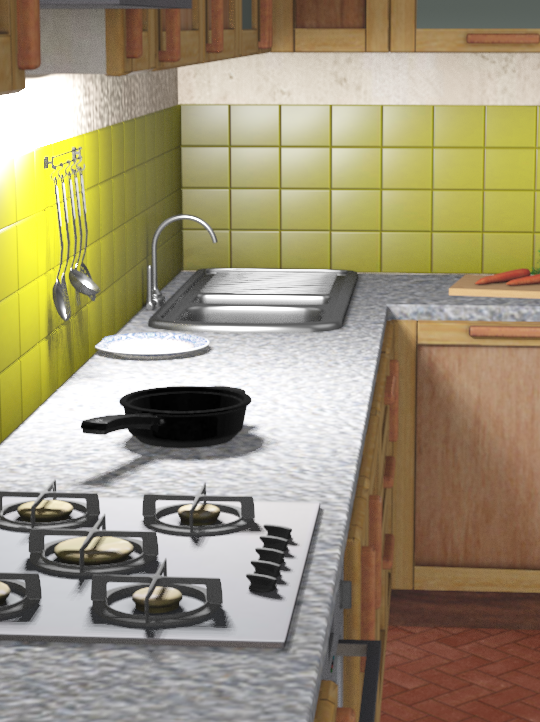
\includegraphics[width=\textwidth]{concept/area_light/kitchen_light_32samples.png}};%
            \spy on ($(initial)+(1.05, -0.3)$) in node at (-0.2, 0.9);
        \end{tikzpicture}
        \caption{32 samples}
    \end{subfigure}
    \begin{subfigure}[b]{0.325\columnwidth}
        \begin{tikzpicture}[spy using outlines={white, circle, magnification=4, size=40, connect spies, every spy on node/.append style={thin}}]
            \node[anchor=center, inner sep=0pt, outer sep=0pt](initial) {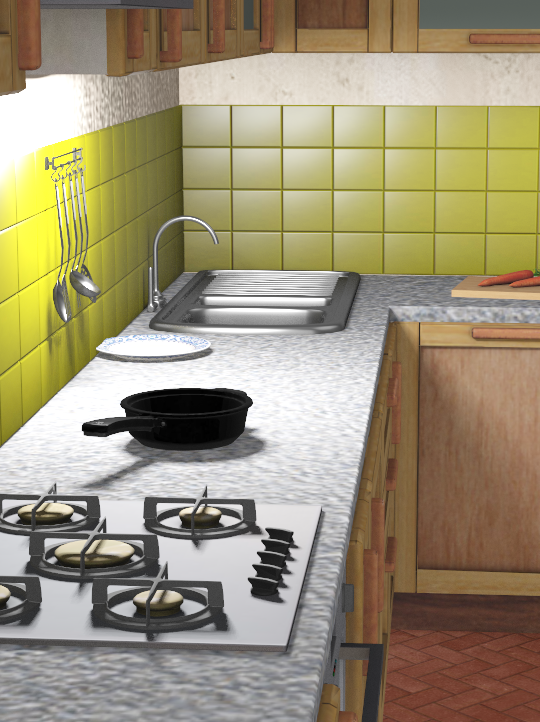
\includegraphics[width=\textwidth]{concept/area_light/kitchen_light_64samples.png}};%
            \spy on ($(initial)+(1.05, -0.3)$) in node at (-0.2, 0.9);
        \end{tikzpicture}
        \caption{64 samples}
    \end{subfigure}
    
    \vspace{-1.2em}
    \caption{Kitchen scene lit by one area light using different sample counts. With 4 samples, the penumbra has an incorrect size. With 16 to 24 samples it is more accurate, but banding artifacts might remain. At 64 samples banding artifacts are gone and the penumbra has the physically correct size.}
    \label{fig:penumbra_rendering}
\end{figure}

To render penumbras using progressive rendering, \cite{limberger2016progressive} have shown that repeated sampling of a light source over multiple frames yields believable results.
We use this approach in order to approximate physically correct shadowing.
We take $n$ samples of equation \ref{math:direct_light_approx}:
\begin{align}
    L_o^{d_i}(p, \omega_o) &\approx \frac{1}{n} \sum_{k=1}^n V(p, \omega_k) f(\omega_o, \omega_r) \frac{\phi_A}{4 \pi d^2} \left|\cos \theta_i\right|,
\end{align}
where $V(p, \omega_k)$ is a visibility function using a sample $\omega_k$ on the area light source.
To approximate this visibility function, we use shadow mapping, where the viewpoint of the light is changed for every sample according to the sample $\omega_k$.
Therefore, within the penumbra of the light, some samples are evaluated as occluded by the shadow mapping algorithm, while others are not.
Thus, when the result is aggregated the penumbra is correctly partially shadowed.
The visual impact of the number of samples is displayed in Figure~\ref{fig:penumbra_rendering}.
In order to reduce jittering across subsequent intermediate frames, it is useful to sort the samples from nearest to furthest from the center of the light source.
Then, during progressive rendering first the samples with low discrepancy will be rendered and slowly more outwards samples are evaluated.
Thus, the penumbras will slowly appear instead of shadows rapidly changing from frame to frame.
In order to render multiple lights, let there be $m$ number of intermediate frames and $n_i$ number of samples for the light with index $i$.
The samples for this light are weighted with $w_i = \frac{m}{n_i}$ in order to be correctly represented in the final rendering.

\subsection{Workload Distribution}
\label{subsec:workload_distribution}
We will now discuss a strategy to distribute respective lighting samples across intermediate frames.
The sampling strategy should meet the following goals:
\begin{enumerate}
    \item The result is physically accurate.
    \item The first frame can be rendered fast and represents the scene sufficiently accurate in order to enable navigation.
    \item The progressive rendering is temporally coherent, i.e., there are no major temporal artifacts.
    \item The sample count is adjustable and allows to favor quality or speed to account for different device capabilities.
\end{enumerate}
We propose handling the first frame differently from subsequent ones by only applying environment lighting during this frame.
This way, environment lighting is used as a mean to illuminate all parts of the scene at a similar level.
While lighting from direct light sources is missing, the material properties are still visible when just lit by the environment and users can track their position within the scene.
Since the environment lighting is cheap to calculate, especially when skipping occlusion evaluation, this speeds up calculation of the first frame.
Furthermore, calculation of shadow maps and depth and normal buffers can be skipped with this approach, which further speeds up calculation.

From the set of all samples $s$, we want to generate subsets $s_i$ which contain all samples that will be calculated during intermediate frame $i$.
Ideally, these subsets should be similar in regard to how much processing power is required to calculate the contained samples.
We introduce the concept of a \emph{sample distributor}, which generates the sets $s_i$ and issues these on requests to the renderer.
With this concept, arbitrary ways to distribute samples over the course of a frame can be implemented. 
Let $s_d$ be a set of all direct lighting samples and $s_e$ a set of all environment samples calculated during a frame.
We distribute $s_e$ uniformly over the whole frame to make sure that there is an even, balanced amount of lighting across all intermediate frames.
While the samples $s_d$ should be distributed uniformly as well, we only start to evaluate them after a brief delay.
This ensures that direct lighting samples, which can differ a lot from one another, do not cause flickering while the user navigates.
We propose the following distribution of samples:
\begin{algorithm}[H]
\begin{algorithmic}
\Function{DistributeSamples}{$samples, startIndex, endIndex$} 
    \State $numFrames \gets endIndex - startIndex$
    \State $framesPerSamples \gets \frac{numFrames}{length(samples)}$
    \State $currentIndex \gets startIndex$
    \ForAll{sample in samples}
        \State $i \gets \left \lfloor{currentIndex}\right \rfloor$
        \State $s_i \gets s_i \cap \{ sample \}$
        \State $currentIndex \gets currentIndex + framesPerSamples$
    \EndFor
\EndFunction
\end{algorithmic}
\caption{Distribution of samples over the course of a frame.}
\end{algorithm}
\noindent
Thus, a set of samples can be distributed within a range of intermediate frames, given the range's start and end index.
With $m$ being the number of intermediate frames, we can calculate \textsc{DistributeSamples}($s_e, 1, m$) and \textsc{DistributeSamples}($s_d, m \cdot f_d, m$), where $f_d$ is the fraction of intermediate frames after that direct light samples start to be evaluated.

\section{Implementation}
\label{sec:implementation}

\begin{figure}
    \centering
    \begin{subfigure}[b]{0.325\columnwidth}
        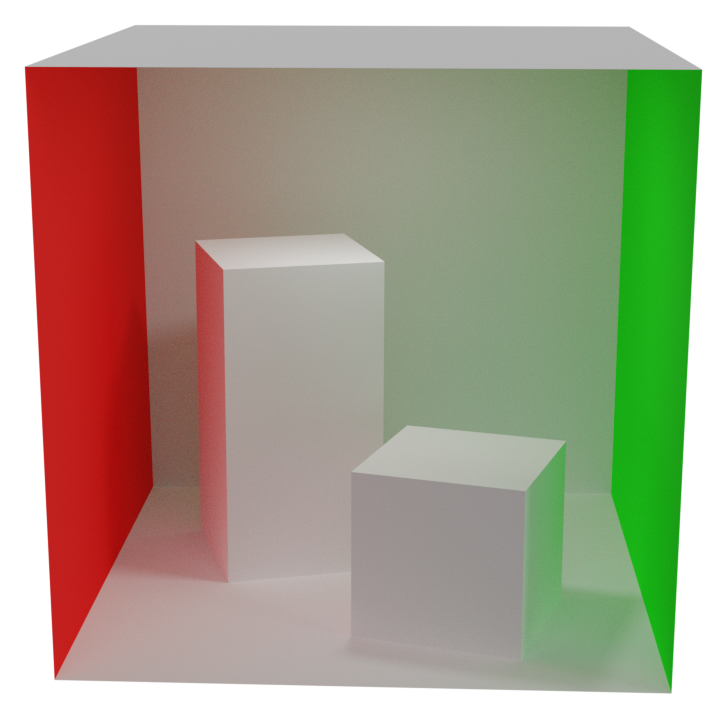
\includegraphics[width=\textwidth]{evaluation/result/cornell_cycles.png}
        \caption{Blender Cycles}
    \end{subfigure} 
    \begin{subfigure}[b]{0.325\columnwidth}
        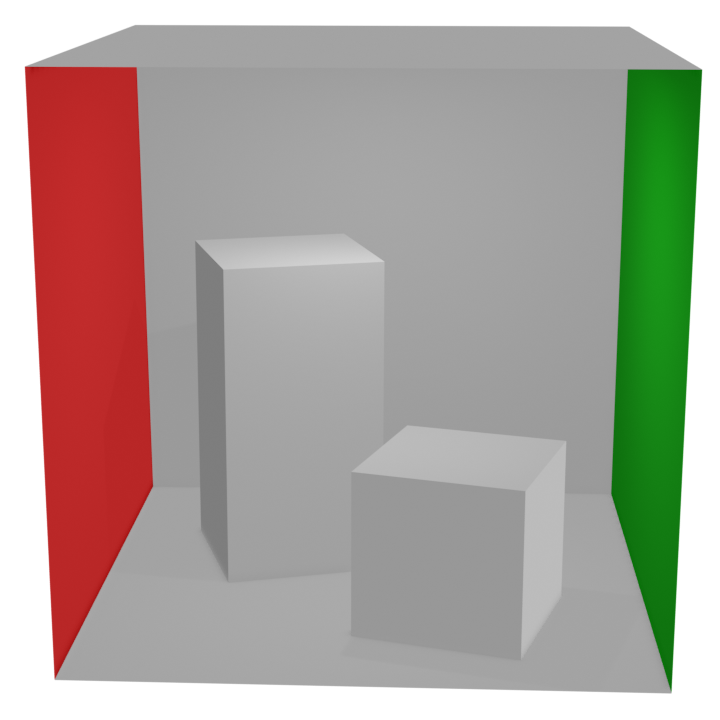
\includegraphics[clip,width=\textwidth]{evaluation/result/cornell_eevee.png}
        \caption{Blender Eevee}
    \end{subfigure} 
    \begin{subfigure}[b]{0.325\columnwidth}
        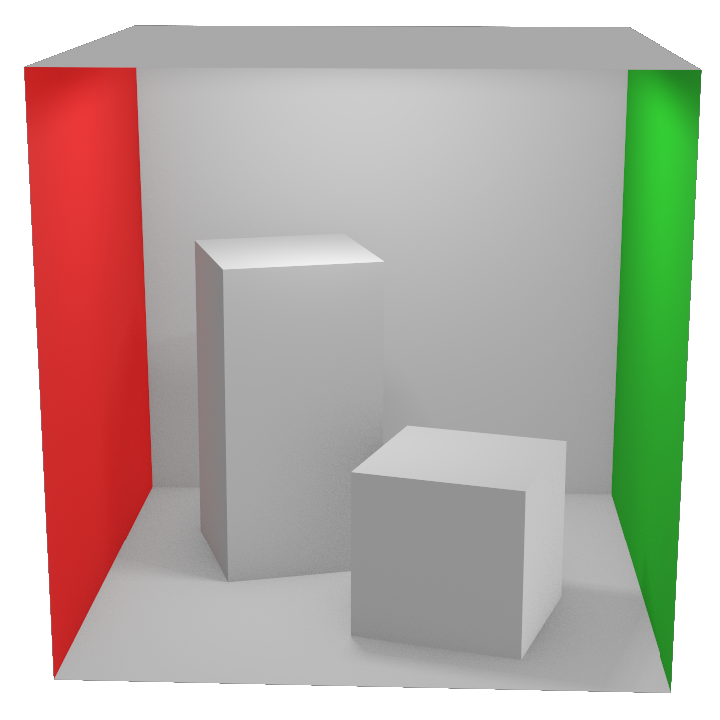
\includegraphics[clip,width=\textwidth]{evaluation/result/cornell_thesis.png}
        \caption{Our renderer}
    \end{subfigure}

    \vspace{-1.2em}
    \caption{Rendering result for the Cornell box test scene.}
    \label{fig:eval_cornell_box}
\end{figure}

\begin{figure*}
    \centering
    \begin{subfigure}[b]{0.325\textwidth}
        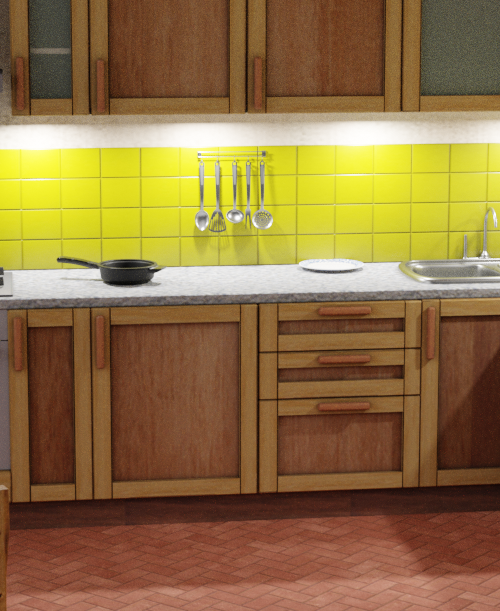
\includegraphics[width=\textwidth]{evaluation/result/kitchen1_cycles1024samples_c.png}
        \caption{Blender Cycles (1024 samples)}
    \end{subfigure} 
    \begin{subfigure}[b]{0.325\textwidth}
        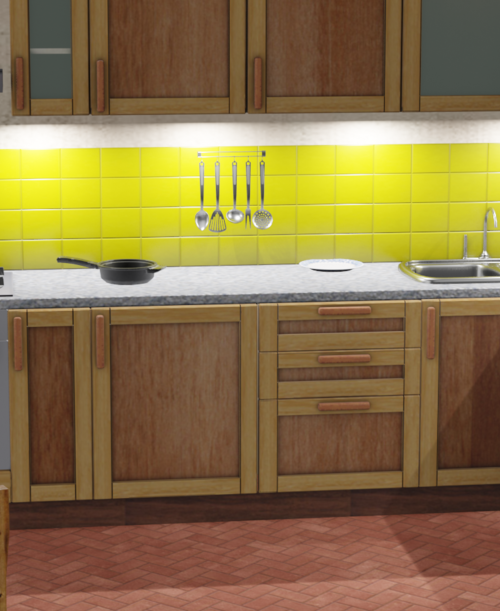
\includegraphics[width=\textwidth]{evaluation/result/kitchen1_eevee_c.png}
        \caption{Blender Eevee (64)}
    \end{subfigure} 
    \begin{subfigure}[b]{0.325\textwidth}
        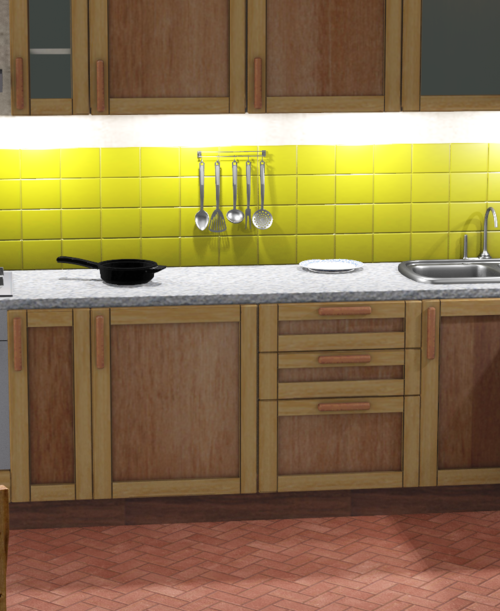
\includegraphics[width=\textwidth]{evaluation/result/kitchen1_thesis256samples_c.png}
        \caption{Our renderer (256 samples)}
    \end{subfigure}
    
    \vspace{-1.2em}
    \caption{Rendering result for the kitchen test scene.}
    \label{fig:eval_kitchen1}
\end{figure*}

We implemented the techniques and sampling strategies described in this work in order to verify and evaluate them.
The implementation is built on top of the library \textit{webgl-operate}\footnote{\url{https://webgl-operate.org/}} and written in \textit{TypeScript}\footnote{\url{https://www.typescriptlang.org/}}.
webgl-operate exposes interfaces to develop robust industry applications using WebGL. 
It does not enforce or favor any specific rendering approach and, furthermore, uses a generalized rendering loop that allows for continuous and progressive rendering control equally.
Therefore, it is a good fit to evaluate our techniques on various devices:
WebGL is available on desktops, tablets, smartphones, and other devices and support for it is growing\footnote{\url{https://caniuse.com/\#feat=webgl2}}.
Another benefit of webgl-operate is that tasks such as context creation, creation of WebGL objects, or fetching textures from remote URLs are encapsulated inside the library.
Additionally, common rendering concepts such as \emph{shadow mapping} can be easily used and extended due to the components already available.

We target WebGL 2.0 as it is supported on a wide range of devices and it ensures that rendering to floating point buffers is supported.
This is necessary, as weighting samples in intermediate frames in combination with supporting high dynamic range rendering can lead to arbitrarily high values stored in buffers.
Therefore, all rendering steps prior to applying tone mapping \cite{salih2012tone} in a post-processing pass are rendered to \texttt{gl.FLOAT} buffers.
Only the result of this post-processing step is stored in a \texttt{gl.RGBA8} buffer, which is copied to the back buffer continuously for presentation to the user.

The rendering workflow is implemented in the following way.
The first frame is rendered as a special case as described in Subsection \ref{subsec:workload_distribution}, where only environment lighting is calculated.
In each subsequent frame, environment and direct lighting samples are drawn from the sample distributor.
These are evaluated during a forward rendering of the scene geometry.
During the second frame, a normal and depth buffer is rendered, which is used for calculating occlusion effects.
For each direct lighting sample, a shadow map is rendered prior to the main rendering pass to calculated shadowing for that sample.
For each environment lighting sample, the diffuse or specular pre-filtered environment map is sampled and occlusion for this sample is calculated as described in Subsection \ref{subsec:occlusion}.

\section{Evaluation}
To validate our techniques, we compare rendering results with the results of two renderers included in the 3D modelling toolkit Blender.
We use the path tracer \emph{Cycles} as a reference renderer to produce photo-realistic comparison results and the rasterizer \emph{Eevee} as a representative modern rasterizer.
We considered comparison to the progressive renderer of SketchFab\footnote{\url{https://sketchfab.com/}} and the physically-based WebGL renderers by Unity\footnote{\url{https://unity.com/}} and the Unreal Engine\footnote{\url{https://www.unrealengine.com/}}.
However, their support for lighting is limited and especially area lights are missing.
We chose 3 scenes from Sketchfab for the evaluation: the \href{https://skfb.ly/6CtVz}{\emph{Cornell box}} by Paul, an \href{https://skfb.ly/6tPpI}{\emph{Italian kitchen}} by F. Coldesina, and a \href{https://skfb.ly/6CtVz}{\emph{Nissan Skyline}} by G. Rodriguez.

\begin{figure*}
    \centering
    \begin{subfigure}[b]{0.325\textwidth}
        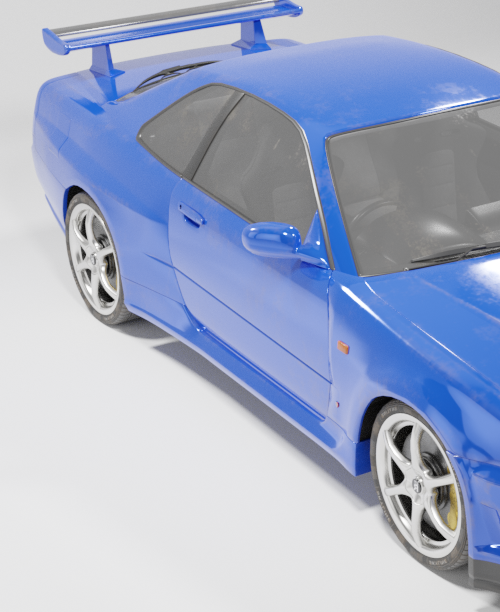
\includegraphics[width=\textwidth]{evaluation/result/skyline1_cycles1024samples_c.png}
        \caption{Blender Cycles (1024)}
    \end{subfigure} 
    \begin{subfigure}[b]{0.325\textwidth}
        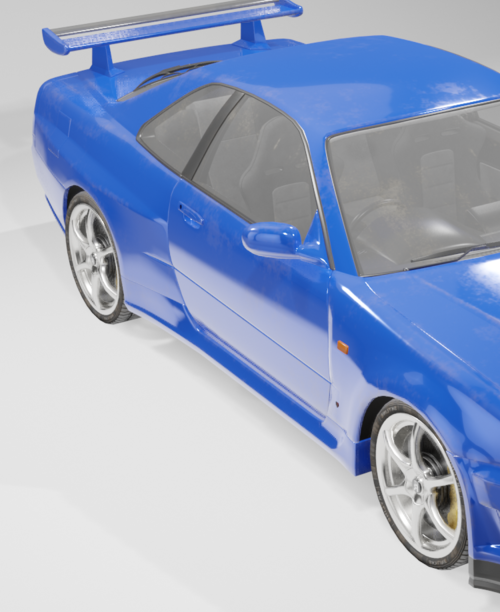
\includegraphics[width=\textwidth]{evaluation/result/skyline1_eevee64samples_c.png}
        \caption{Blender Eevee (64)}
    \end{subfigure} 
    \begin{subfigure}[b]{0.325\textwidth}
        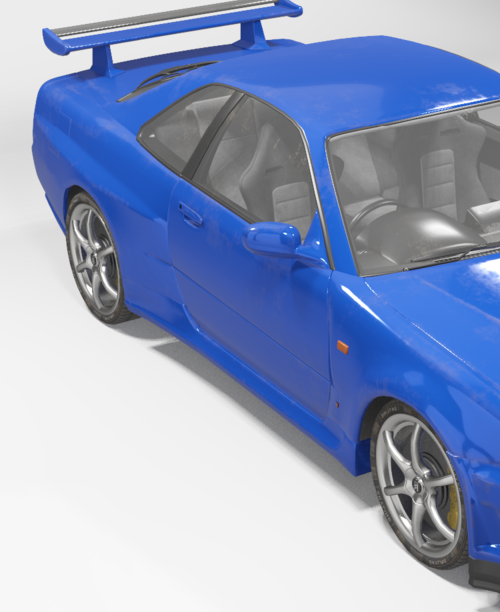
\includegraphics[width=\textwidth]{evaluation/result/skyline1_thesis256samples_c.png}
        \caption{Our renderer (256)}
    \end{subfigure}

    \vspace{-1.2em}
    \caption{Rendering result for the Skyline (car) test scene.}
    \label{fig:eval_skyline1}
\end{figure*}

\subsection{Evaluation of Visual Rendering Quality}
\label{subsec:rendering_result}
The renderings of the Cornell box can be seen in Figure~\ref{fig:eval_cornell_box}.
The path-traced reference show a high amount of diffuse indirect lighting, especially at the back wall and the sides of the boxes.
The two rasterizers lack this indirect lighting.
The top light causes penumbras (soft shadows) from the two boxes which are not present in the Eevee rendering.
In comparison, our renderer captures the shape of the shadows and matches the size of their penumbras closely to the path-traced reference.
The intensity of the shadow is a bit lower compared to the reference, but more visible than in the Eevee rendering.
Our progressive technique cannot perfectly capture diffuse light bounces, but handles light intensity and shadowing appropriately w.r.t. the reference in general.

The rendering results for the kitchen scene are shown in Figure~\ref{fig:eval_kitchen1}.
In the Cycles reference we can observe mostly direct lighting by six area lights above the kitchen counter.
Due to multiple lights being present, we have multiple soft shadows and widening penumbras across the wooden drawers.
The Eevee rendering does not correctly capture shadowing in all parts of the scene.
Most notably, the shadowing of the kitchen utensils and the pan are not appropriately covered.
Also the size of the penumbra on the floor is not correctly captured by the Eevee rendering.
Again, our renderer matches the size and intensity of the shadows accurately and yields penumbras that are indistinguishable from the reference (without the noise).

The renderings for the Skyline (car) model are shown in Figure \ref{fig:eval_skyline1}.
We can see a high amount of reflection on the coating, the glass, and the tires.
Because there are four lights placed on all corners of the car, shadowing is only present directly below the vehicle.
Again, the Eevee rendering does not display the correct amount of shadowing.
While the shadows under the car have approximately the correct shape, the intensity of the shadow is much lower than in the reference.
Our renderer captures the shape and intensity of the shadows seen in the reference better than Eevee.
Also, the occlusion details, e.g., at the door handle, are captured better than by the Eevee rendering.
However, the bright reflections of the ground at the side are missing (see future work).

\subsection{Evaluation of Rendering Performance}
In order to measure the rendering speed, we perform tests on three different devices:
\begin{itemize}
    \item A desktop computer with an Intel Core i5-3570K CPU and an AMD Radeon HD 7950 GPU.
    \item A 2013 MacBook Air with an Intel Core i5-4250U CPU and an Intel HD Graphics 5000 GPU.
    \item A Motorola Moto X4 smartphone with a Qualcomm Snapdragon 630 CPU and integrated Adreno 508 GPU.
\end{itemize}

\paragraph{Performance Comparison between Renderers}
\begin{table}[h]
    \centering
    \caption{Rendering time in seconds of the different renderers on a desktop computer (frame count of 128 for ours).}
    \begin{tabular}{l|*{6}{r}}
        & \multicolumn{2}{c}{Cornell Box} & \multicolumn{2}{c}{Skyline} & \multicolumn{2}{c}{Kitchen}\\
        & 720p & 1080p & 720p & 1080p & 720p & 1080p\\\hline
        Cycles & 11:27.63 &   --- & 24:37.75 &   --- & 23:25.81 &   --- \\
        Eevee  &     0.53 &  0.99 &     2.38 &  3.37 &     1.77 &  2.55 \\
        Ours   &     0.19 &  0.41 &     0.65 &  1.39 &     0.82 &  1.68 \\
    \end{tabular}
    \label{tab:performance_different_renderers}
\end{table}
We compare the rendering time off all three renderers for both 1920x1080 (1080p) resolution and 1280x720 (720p) resolution.
For our renderer we use a frame count of 128 for this comparison, while we use a sample count of 64 for Eevee.
For Cycles we use a sample count of 1024 to reduce noise.
The results are shown in Table \ref{tab:performance_different_renderers}.
We can see that path tracing using Cycles takes an order of magnitude more time in comparison to the rasterizers.
Despite being progressive, our renderer is faster than Eevee across all scenes and resolutions.
Even with presenting intermediate results, our final rendering is available faster than using Eevee with 64 samples.

\paragraph{Performance Comparison on different Hardware}
\begin{table}[b]
    \centering
    \caption{Rendering time in seconds of our renderer on different devices using a frame count of 128.}
    \begin{tabular}{l|*{6}{r}}
        & \multicolumn{2}{c}{Cornell Box} & \multicolumn{2}{c}{Skyline} &  \multicolumn{2}{c}{Kitchen}\\
        & 720p & 1080p & 720p & 1080p & 720p & 1080p\\\hline
        Desktop    & 0.19 & 0.41 &  0.65 & 1.39 &  0.82 & 1.68 \\
        Laptop     & 1.26 & 3.21 &  4.58 & 7.52 &  5.44 & 9.85 \\
        Smartphone & 7.47 &  --- & 26.27 &  --- & 32.66 &  ---
    \end{tabular}
    \label{tab:performance_different_devices}
\end{table}
We run our renderer on all three devices using a frame count of 128.
The results are shown in Table \ref{tab:performance_different_devices}.
We can see that rendering in 720p on laptop and desktop reduces rendering time significantly and even cuts the time in half in some cases.
While rendering on the desktop produces results very quickly, on the laptop it takes some seconds to generate the final rendering results, especially on 1080p resolution.
For a progressive renderer, this time is still acceptable because intermediate results are already shown during calculation of the image.
For the smartphone, rendering more complex scenes at 720p resolution and 128 frames is not yet feasible on mid-range smartphones at the moment (about 30 seconds).

\paragraph{Evaluation of Interactivity}
Testing the rendering speed of the first frame for the kitchen scene resulted in 0.98, 1.28, and 11.02 milliseconds on desktop, laptop, and smartphone respectively (720p).
The rendering speed is within the single digit millisecond range for both the desktop and laptop at 720p and 1080p resolution.
On the smartphone we still reach an interactive rendering speed of below 16 ms.
This shows that our progressive rendering with its workload distribution manages to keep the rendering time for the first frame very low.

\section{Conclusion and Future Work}

\begin{figure*}[t]
    \centering
    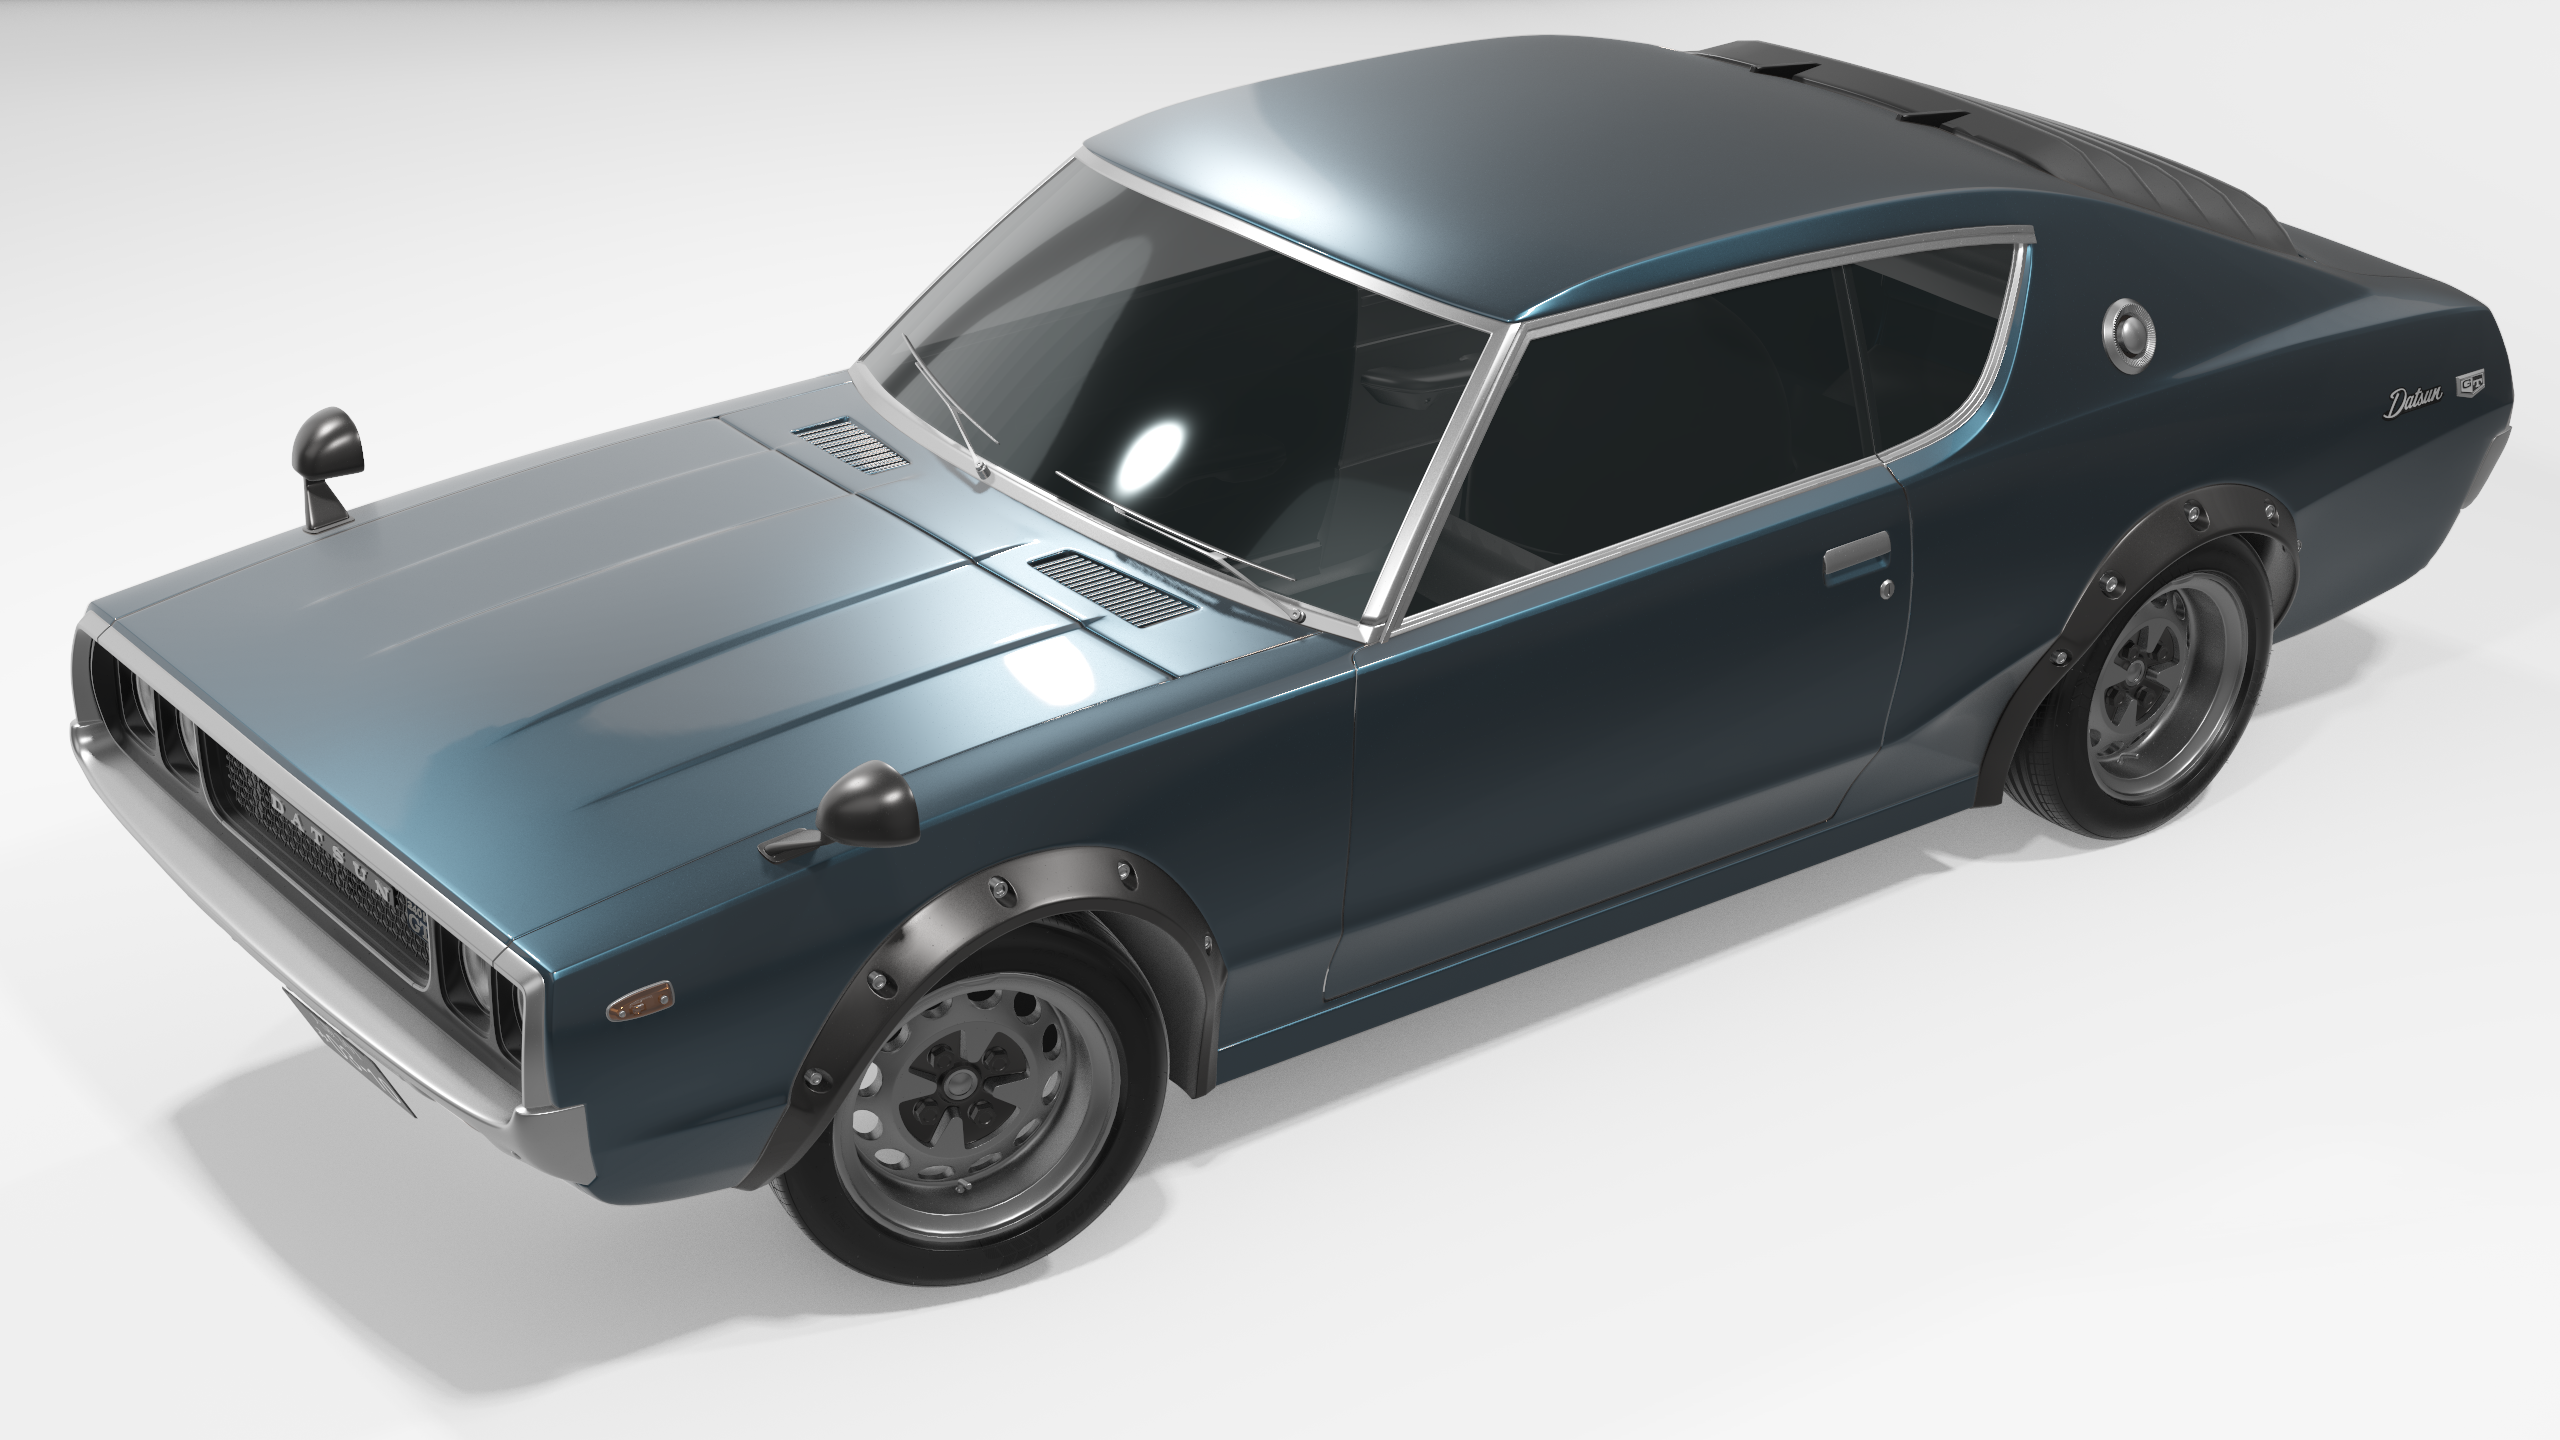
\includegraphics[width=\linewidth]{evaluation/result/datsun}
    \vspace*{-1.2em}
    \caption{Our prototypical implementation available at \href{p-otto.waduhek.de/demos/progressive-lighting.html}{https://p-otto.waduhek.de/demos/progressive-lighting.html}. We are currently adding on screen-space reflections and depth-of-field to the renderer. 3D Model: \href{https://skfb.ly/6u6VR}{\emph{Datsun 240k GT}} by Karol Miklas}.
    \label{fig:result_datsun}
\end{figure*} 

In this work, rendering techniques and sampling strategies for lighting 3D scenes using progressive rendering were presented.
Using an implementation within a web-based renderer, we showed that lighting and shadowing is physically believable, while achieving interactivity even on mobile devices.
For further work, a mechanism to automatically adapt sample counts and strategies depending on the performance of the rendering device could be explored.
Using an adaptive mechanism could push increase the quality of rendering on desktop devices and favor interactivity on mobile hardware.
Additionally, a progressive implementation of screen-space reflections would enable specular bounces within the scene, currently not captured by our renderer.

\begin{acks}
This work is part of the “Software-DNA” project, funded by the European Regional Development Fund (EFRE) and the State of Brandenburg (ILB).
\end{acks}

\bibliographystyle{ACM-Reference-Format}
\bibliography{references}

\end{document}
\endinput
